\chapter{Fonctions usuelles}
\label{chap:fonctionsusuelles}
\minitoc
\minilof
\minilot
%
Vous connaissez depuis la classe de Terminale les fonctions trigonométriques, l’exponentielle et le logarithme népérien. Notre premier objectif sera de démontrer rigoureusement leurs propriétés. Nous introduirons aussi les fonctions hyperboliques ainsi que les fonctions réciproques des fonctions trigonométriques et hyperboliques. Pour comprendre quelques démonstrations, vous aurez besoin des notions de base de l’analyse~: limites, continuité, dérivabilité et convexité. Quelques théorèmes sont donnés dans l'annexe~\ref{chap:theogen}.
%
\section{Logarithmes \& exponentielles}
\label{sec:chap1-logetexp}
%
\subsection{Logarithme népérien}
\label{subsec:chap1-lognep}
%
\begin{defdef}
\label{def:chap1-deflognep}
On appelle la fonction logarithme népérien l'unique primitive de la fonction inverse \footnote{qui est continue sur \(\Rplusetoile\)} qui s'annule en \(1\). On a donc pour tout \(x\) strictement positif
\begin{equation}
  \ln x=\int_{1}^{x} \frac{\diff t}{t}.
\end{equation}
\end{defdef}
%
Ainsi, par définition, on a~:
\begin{itemize}
\item \(\ln 1 = 0\);
\item \(\ln\) est dérivable sur \(\Rplusetoile\);
\item la dérivée du logarithme népérien est telle que pour tout \(x>0\), \(\ln'(x)=\frac{1}{x}\).
\end{itemize}
Le logarithme népérien est indéfiniment dérivable et strictement croissant.
%
\begin{theo}
\label{theo:lognep1}
  Pour tout \(x, y \in \Rplusetoile\), on a
  \begin{equation}
    \ln(xy)=\ln x + \ln y.
  \end{equation}
\end{theo}
\begin{proof}
  Soit \(y \in \Rplusetoile\) fixé. On définit la fonction
  \begin{equation}
    \fonction{f_y}{\Rplusetoile}{\R}{x}{\ln(xy)},
  \end{equation}
  alors \(f_y\) est dérivable sur \(\Rplusetoile\) par produit et composition de fonctions qui le sont. En dérivant la fonction \(f_y\), on a pour tout \(x \in \Rplusetoile\)
   \begin{equation}
     f_y'(x)=y \frac{1}{xy}=\frac{1}{x}=\ln' x.
   \end{equation}
  Il existe donc une constante réelle \(c\) telle que
  \begin{equation}
    f_y(x)=\ln(xy)=\ln x + c.
  \end{equation}
  Or \(f_y(1)=\ln(y)=c\).
\end{proof}
%
\begin{prop}
  Soient \(x, y \in \Rplusetoile\) et \(n \in \Z\), alors les égalités suivantes sont vraies~:
  \begin{gather}
    \ln \left(\frac{1}{x}\right)=-\ln x;\\
    \ln \left(\frac{x}{y}\right)=\ln x - \ln y; \\
    \ln x^n=n\ln x.
  \end{gather}
\end{prop}
\begin{proof}
  \begin{itemize}
  \item \( 0 = \ln 1 = \ln \left(\frac{1}{x} \cdot x \right) = \ln \left(\frac{1}{x}\right) + \ln x \).
  \item \( \ln \left(\frac{x}{y}\right)=\ln x + \ln \left(\frac{1}{y}\right)=\ln x - \ln y\).
  \item On montre la proposition par récurrence sur \(n\)~:
    \begin{itemize}
    \item On a \(\ln(x^0) = 0 = 0 \cdot \ln(x)\).
    \item Ensuite, supposons la propriété vraie au rang \(n\), montrons qu'elle est vraie au rang \(n+1\)~:
      \begin{equation}
        \ln x^{n+1} = \ln x + \ln x^n = \ln x + n \cdot \ln x = (n+1) \ln x.
      \end{equation}
      Par théorème de récurrence, la proposition est vraie pour tous les entiers naturels.
    \item Montrons le pour les entiers négatifs. Si \(n \in \Z\setminus\N\), alors
      \begin{equation}
        \ln x^n = -\ln x^{-n}=-(-n\ln x)=n\ln x.
      \end{equation}
    \end{itemize}
  \end{itemize}
\end{proof}
%
\begin{theo}
\label{theo:limln}
  La fonction logarithme népérien vérifie les limites suivantes~:
  \begin{gather}
    \lim\limits_{x \to + \infty} \ln x = +\infty; \\
    \lim\limits_{x \to 0^{+}} \ln x = -\infty;\\
    \lim\limits_{x \to 1} \frac{\ln x}{x-1}=1.
  \end{gather}
\end{theo}
\begin{proof}
  \begin{itemize}
  \item L'application logarithme népérien est strictement croissante. Pour tout naturel \(n\), on a \(\ln 2^n = n \ln 2\). De plus \(\ln 2 >0\) donc \(\lim\limits_{n \to \infty} \ln 2^n = + \infty\). La fonction logarithme népérien n'est pas majorée et comme elle est croissante, on en déduit que \(\lim\limits_{x \to \infty} \ln x = +\infty\).
  \item Puisque \(\ln x = - \ln\left(\frac{1}{x}\right)\), alors lorsque \(x\to 0^+\), \(\frac{1}{x} \to + \infty\). Donc \(\ln \left(\frac{1}{x}\right) \to +\infty\) et ainsi \(\lim\limits_{x \to 0^+} \ln x = - \infty\).
  \item Ce rapport est le taux d'accroissement de la fonction logarithme népérien en \(1\). La limite est donc la dérivée de \(\ln\) en \(1\). C'est à dire \(\left.\frac{1}{x}\right)_{x=1}=1\).
  \end{itemize}
\end{proof}
%
\begin{figure}
  \centering
  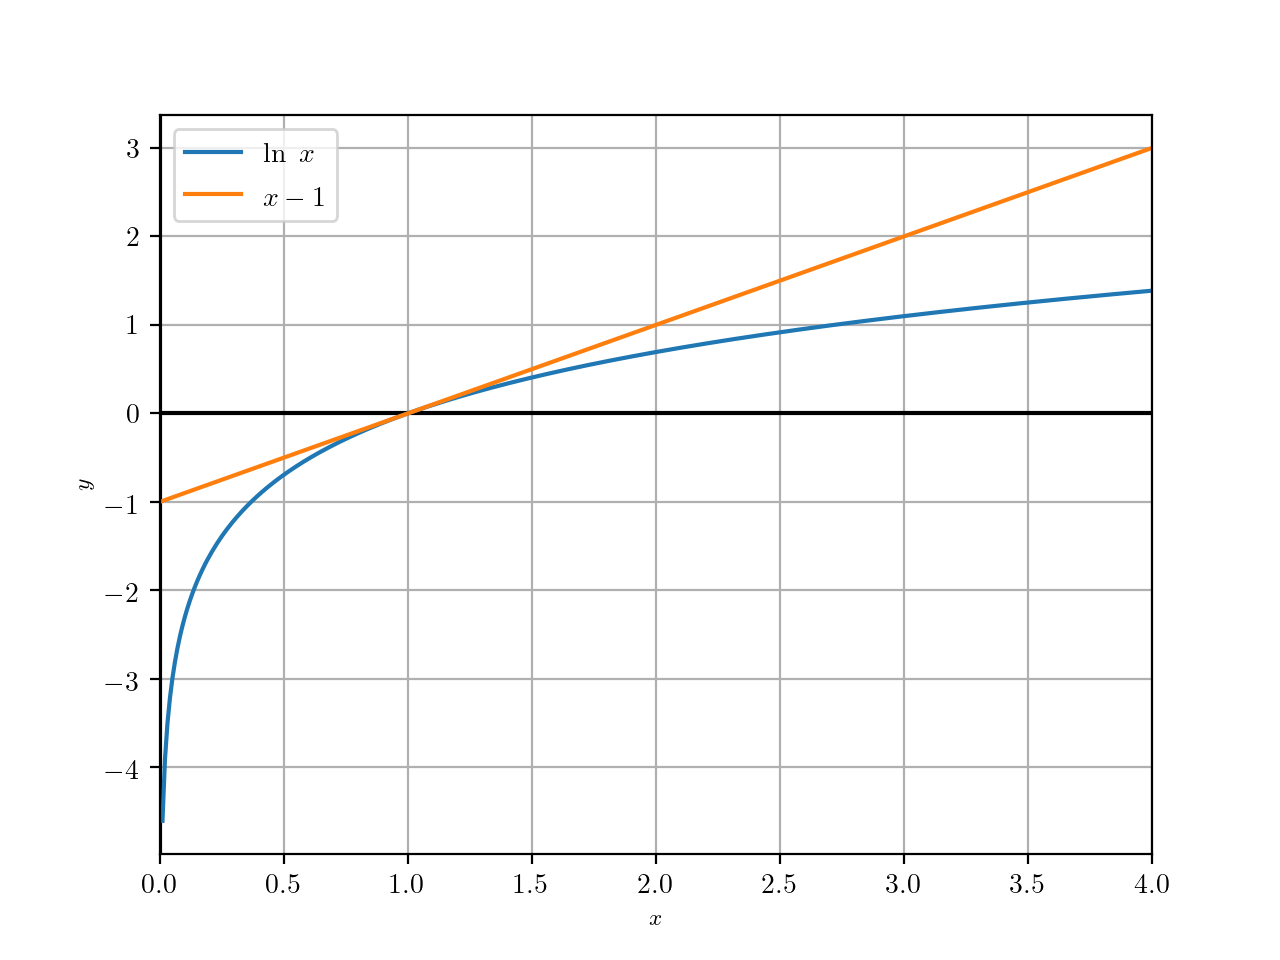
\includegraphics[scale=0.6]{lognep.png}
  \caption{Tracé du logarithme népérien}
  \label{fig:traceln}
\end{figure}
%
\begin{theo}
  L'ensemble \(E\) des fonctions dérivables de \(\R^{\Rplusetoile}\) telles que~:
  \begin{equation}
    \label{eq:fonclog}
    \forall x, y \in \Rplusetoile \quad f(xy)=f(x)+f(y)
  \end{equation}
  est la droite vectorielle engendrée par le logarithme népérien, c'est-à-dire que~:
  \begin{equation}
    E=\enstq{\fonction{f_{\alpha}}{\Rplusetoile}{\R}{x}{\alpha \ln x}}{\alpha \in \R}.
  \end{equation}
\end{theo}
\begin{proof}
  Soit une fonction \(f \in \R^{\Rplusetoile}\) dérivable sur \(\Rplusetoile\) vérifiant l'équation~\eqref{eq:fonclog}. Comme \(f\) est dérivable, on peut dériver l'équation~\eqref{eq:fonclog} par rapport à \(x\) et on obtient pour tout \(y\) strictement positif
  \begin{equation}
    y f'(xy)=f'(x).
  \end{equation}
  Pour \(x=1\), on a
  \begin{equation}
    y f'(y)=f'(1),
  \end{equation}
  c'est-à-dire \(f'(y)=f'(1) \ln' y\). Donc en intégrant cette équation à partir de \(1\), on a
  \begin{equation}
    f(y)=f'(1)\ln y + f(1).
  \end{equation}
  En appliquant l'équation~\eqref{eq:fonclog} en \(x=y=1\), on a \(f(1)=2f(1)\) donc \(f(1)=0\).

  On a montré que si une fonction \(f\) de \(\R^{\Rplusetoile}\) dérivable vérifie l'équation~\eqref{eq:fonclog}, alors elle est proportionnelle au logarithme népérien. La réciproque est due au théorème~\ref{theo:lognep1}.
\end{proof}
%
\subsection{Logarithmes de base a}
\label{subsec:chap1-loga}
\begin{defdef}
  Soit un réel \(a\) de \(\Rplusetoile\setminus\{1\}\). On définit la fonction logarithme de base  \(a\), notée \(\log_a\) par \(\fonction{\log_a}{\Rplusetoile}{\R}{x}{\dfrac{\ln x}{\ln a}}\).
\end{defdef}
%
\begin{prop}
  \begin{itemize}
  \item \(\log_a(1)=0\);
  \item pour tout \(a \in\Rplusetoile\setminus\{1\}\), la fonction \(\log_a\) est dérivable, donc continue, sur \(\Rplusetoile\) et pour tout réel \(x\) strictement positif
    \begin{equation}
      \log_a'(x)=\frac{1}{x \ln a}.
    \end{equation}
  \end{itemize}
\end{prop}
\begin{proof}
  Ce sont des conséquences immédiates de la définition et des propriétés du logarithme népérien.
\end{proof}
%
\begin{prop}
  Soient \(x\) et \(y\) deux réels strictement positifs, \(a\) et \(b\) deux bases de logarithme~\footnote{Une base de logarithme est un réel strictement positif différent de 1}, alors~:
  \begin{gather}
    \log_a xy=\log_a x + \log_a y; \\
    \log_b x=\log_ba \log_ax; \\
    \log_{1/a} x=-\log_a x.
  \end{gather}
\end{prop}
\begin{proof}
  \begin{itemize}
  \item \(\log_a xy= \frac{\ln xy}{\ln a}= \frac{\ln x}{\ln a} +\frac{\ln y}{\ln a}=\log_ax+\log_ay\);
  \item \(\log_b x = \frac{\ln x}{\ln b}=\frac{\ln x}{\ln a} \times \frac{\ln a}{\ln b}=\log_ax \log_ba\);
  \item soit en prenant \(b=\frac{1}{a} \in \Rplusetoile-\{1\}\) alors \(\log_{\frac{1}{a}}x=\log_ax \log_{\frac{1}{a}}(a)=\log_ax \frac{\ln a}{-\ln a}=-\log_ax\).
  \end{itemize}
\end{proof}
Le logarithme décimal en base \(10\) et le logarithme binaire en base \(2\).
\begin{figure}
  \centering
  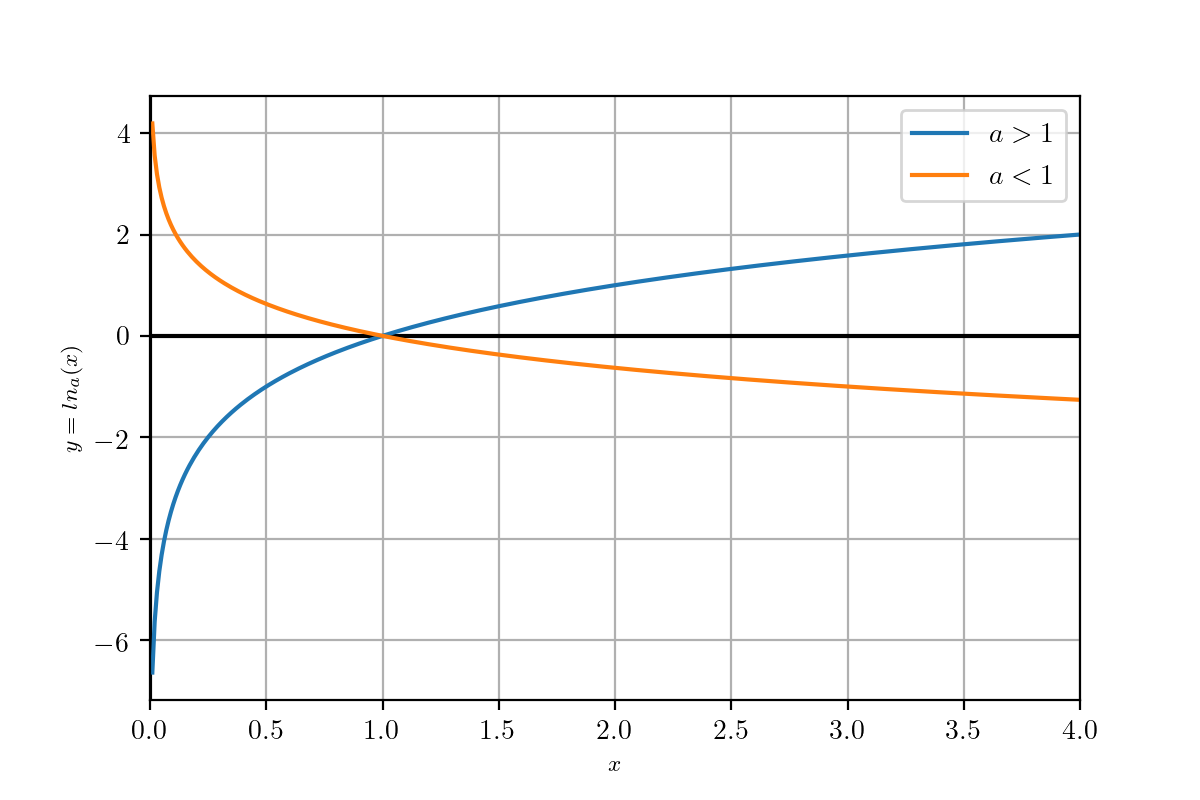
\includegraphics[scale=0.6]{logbase.png}
  \caption{Tracé des logarithmes de bases quelconque}
  \label{fig:traceloga}
\end{figure}
\subsection{Exponentielle}
\label{subsec:chap1-exp}
\begin{defdef}
  L'application logarithme népérien est continue sur \(\Rplusetoile\) et strictement croissante, telle que \(\lim\limits_{0^+} \ln =-\infty\) et \(\lim\limits_{+\infty} \ln = +\infty\). Alors le logarithme népérien induit une bijection de \(\Rplusetoile\) sur \(\R\). L'application réciproque du logarithme népérien est la fonction exponentielle notée \(\exp\) telle que
  \begin{equation}
    \fonction{\exp}{\R}{\Rplusetoile}{x}{\exp(x)}.
  \end{equation}
\end{defdef}
%
\begin{prop} Les fonctions logarithme népérien et exponentielle vérifient
  \begin{equation}
    \forall (x,y) \in \R \times \Rplusetoile \quad y=\exp(x) \iff x=\ln y.
  \end{equation}
\end{prop}
\begin{proof}
  C'est une conséquence de la définition.
\end{proof}
%
\begin{prop}
  La fonction exponentielle est dérivable sur \(\R\) et
  \begin{equation}
    \forall x \in \R \quad \exp'(x)=\exp(x).
  \end{equation}
\end{prop}
\begin{proof}
  La fonction \(\ln\) est dérivable sur \(\Rplusetoile\) et pour tout réel \(y\), \(\exp(y)>0\). Alors d'après les théorèmes généraux~\footnote{cf.\ annexe~\ref{chap:theogen}}, on a
  \begin{equation}
    \exp'(y)=\frac{1}{\ln'(\exp(y))}=\exp(y).
  \end{equation}
\end{proof}
%
\begin{prop} \label{prop-chap1:addexp}
  \begin{equation}
    \forall x, y \in \R \quad \exp(x+y)=\exp(x) \cdot \exp(y).
  \end{equation}
On dira plus tard que c'est un morphisme de groupes du  groupe additif \((\R,+)\) sur le groupe multiplicatif \((\R^*,\times)\)~\footnote{cf.\ chapitre~\ref{chap:groupes}}.

\end{prop}
\begin{proof}
  Soient deux réels \(x\) et \(y\). Comme
  \begin{equation}
    \ln(\exp(x+y))=x+y=\ln(\exp(x))+\ln(\exp(y))=\ln(\exp(x) \exp(y)),
  \end{equation}
  en appliquant l'exponentielle~\footnote{L'exponentielle est une fonction bijective} on obtient le résultat.
\end{proof}
%
\begin{prop}
  Soient \(x\) et \(y\) deux réels et un entier relatif \(n\), alors
  \begin{gather}
    \exp(-x)=\frac{1}{\exp(x)}; \\
    \exp(x-y)=\frac{\exp(x)}{\exp(y)}; \\
    \exp(nx)=\exp(x)^n.
  \end{gather}
\end{prop}
\begin{proof}
  \begin{itemize}
  \item \(\ln(\exp(-x))=-x=-\ln(\exp(x))=\ln \left(\frac{1}{\exp(x)}\right)\) et on peut composer par \(\exp\)~\footnote{Idem} pour obtenir le résultat;
  \item \(\exp(x-y)=\exp(x) \exp(-y)=\frac{\exp(x)}{\exp(y)}\);
  \item \(\ln(\exp(nx))=nx=n \ln(\exp(x))=\ln(\exp(x)^n)\) puis en composant par l'exponentielle, on a le résultat.
  \end{itemize}
\end{proof}
%
\begin{prop}
  La fonction exponentielle admet les limites suivantes~:
  \begin{gather}
    \lim\limits_{x \to \infty} \exp(x)=+\infty;\\
    \lim\limits_{x \to -\infty} \exp(x)=0;\\
    \lim\limits_{x \to 0} \frac{\exp(x)-1}{x}=1.
  \end{gather}
\end{prop}
\begin{proof}
  Les deux premières propositions sont des conséquences de la définition et la dernière est la limite du taux d'accroissement en zéro, soit la dérivée en 0 de l'exponentielle.
\end{proof}
%
\begin{figure}
  \centering
  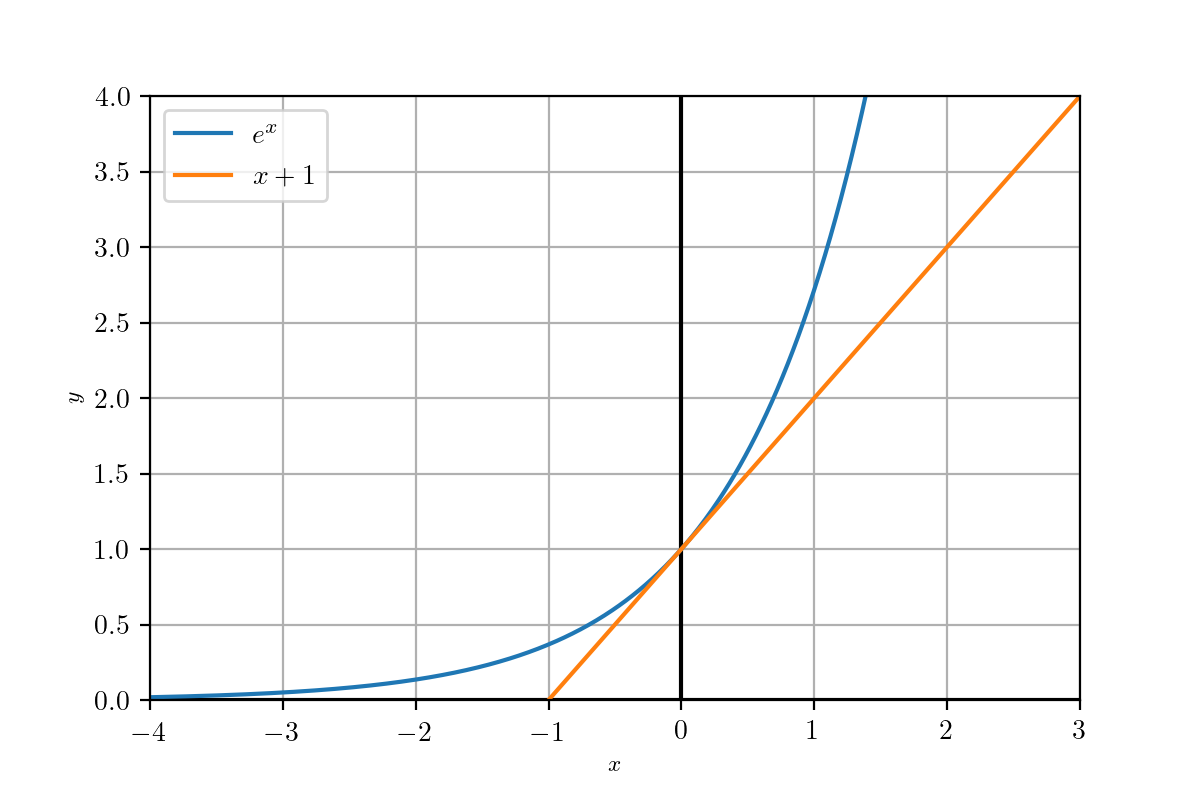
\includegraphics[scale=0.6]{exp.png}
  \caption{Tracé de l'exponentielle}
  \label{fig:traceexp}
\end{figure}
%
\begin{theo}
  L'ensemble \(E\) des fonctions de \(\R^{\R}\) dérivables qui vérifient l'équation
  \begin{equation}
    \label{eq:foncexp}
    \forall x, y \in \R \quad f(x+y)=f(x) \cdot f(y)
  \end{equation}
  est
  \begin{equation}
    E=\left\{0\right\} \cup \enstq{\fonction{g_{\alpha}}{\R}{\R}{x}{\exp(\alpha x)}}{\alpha \in \R}.
  \end{equation}
\end{theo}
\begin{proof}
  Soit une fonction \(f \in \R^{\R}\) dérivable qui vérifie l'équation~\eqref{eq:foncexp}, alors en dérivant cette équation on obtient~:
  \begin{equation}
    \label{eq:foncexpun}
    f'(x+y)=f'(x)f(y)=f(x)f'(y).
  \end{equation}
  Deux cas sont possibles~:
  \begin{itemize}
  \item la fonction nulle est solution,
  \item si la fonction n'est pas nulle, il existe une réel \(x_0\) tel que \(f(x_0) \neq 0\). Alors
    \begin{equation}
      \forall y \in \R \quad f(x_0)= f(x_0-y)f(y).
    \end{equation}
    Soit \(y \in \R\), alors \(f(y) \neq 0\). La fonction \(f\) ne s'annulant donc jamais, on peut reprendre l'équation~\ref{eq:foncexpun} et écrire que
    \begin{equation}
      \label{eq:foncexpdeux}
      \forall x \in \R \quad \frac{f'(x)}{f(x)}=\frac{f'(0)}{f(0)}.
    \end{equation}
    D'après l'équation~\ref{eq:foncexp}, on a
    \begin{equation}
      f(0)=f(0)^2.
    \end{equation}
    Comme \(f\) ne s'annule pas, nécessairement \(f(0)=1\). La fonction \(f\) est donc toujours positive. D'après l'équation~\eqref{eq:foncexpdeux}, il existe un réel \(c\) tel que
    \begin{equation}
      \forall x \in \R \quad \ln \abs{f(x)}=\ln f(x)=f'(0) x + c.
    \end{equation}
    Alors
    \begin{equation}
      f(x)=\exp(f'(0) x +c),
    \end{equation}
    et comme \(f(0)=1\), on a \(c=0\).
  \end{itemize}
  La réciproque est due à la proposition~\ref{prop-chap1:addexp}. Si une fonction est dans \(E\) alors elle vérifie l'équation~\ref{eq:foncexp}.
\end{proof}
%
\subsection{Exponentielles de base a}
\label{subsec:chap1-expa}
\begin{defdef}
  Soit une base \(a\) de logarithme dans \(\Rplusetoile\setminus\{1\}\). Comme l'application logarithme népérien, l'application \(\log_a\) induit une bijection de \(\Rplusetoile\) sur \(\R\) et admet une bijection réciproque appelée exponentielle de base \(a\), notée \(\exp_a\).
\end{defdef}
\begin{prop}
  \begin{equation}
    \forall x \in \R \ \forall y \in \Rplusetoile \ \forall a \in \Rplusetoile\setminus\{1\} \quad y=\exp_a(x) \iff x=\log_a(y).
  \end{equation}
\end{prop}
\begin{proof}
  C'est une conséquence directe de la définition.
\end{proof}
%
\begin{prop}
  \begin{equation}
    \forall x \in \R \ \forall a \in \Rplusetoile\setminus\{1\} \quad \exp_a(x)=\exp(a\ln x).
  \end{equation}
\end{prop}
\begin{proof}
  On sait que~:
  \begin{equation}
    \log_a(\exp_a(x))=x=\frac{\ln(\exp(x \ln a))}{\ln a}=\log_a(\exp(x \ln a)),
  \end{equation}
  et en appliquant \(\exp_a\), qui est bijective, on obtient le résultat.
\end{proof}
%
\begin{prop}
  Soient \(a\) une base de logarithme, \(x\) et \(y\) deux réels et \(n\) un entier relatif. Alors les propriétés suivantes sont vraies~: la fonction \(\exp_a\) est indéfiniment dérivable sur \(\R\) et
  \begin{equation}
    \forall x \in \R \quad \exp_a'(x)=\ln a \exp_a(x).
  \end{equation}
 De plus~:
  \begin{gather}
    \exp_a(x+y)=\exp_a(x) \exp_a(y); \\
    \exp_a(-x)=\frac{1}{\exp_a(x)}; \\
    \exp_a(x-y)=\frac{\exp_a(x)}{\exp_a(y)}; \\
    \exp_a(nx)=\exp_a(x)^n;\\
    \exp_{\frac{1}{a}}(x)=\exp(-x \ln a)=\exp_a(-x).
  \end{gather}
\end{prop}
\begin{proof}
  Ce sont des conséquences immédiates des propriétés de l'exponentielle.
\end{proof}
%
En appliquant la formule précédente en \(x=1\), et on a~: \(\exp_a(n)=\exp_a(1)^n=a^n\). Alors on pose
\begin{equation}
  \forall x \in \R \quad a^x=\exp_a(x)=\exp(x \ln a)
\end{equation}
En particulier pour l'exponentielle~: \(\e^x=\exp(x)\). On pose aussi que pour tout réel \(x\), \(1^x=1\). Donc \(\forall a>0 \ \forall x>0 \quad a^x=\exp(x \ln a)\).
%
\begin{figure}
  \centering
  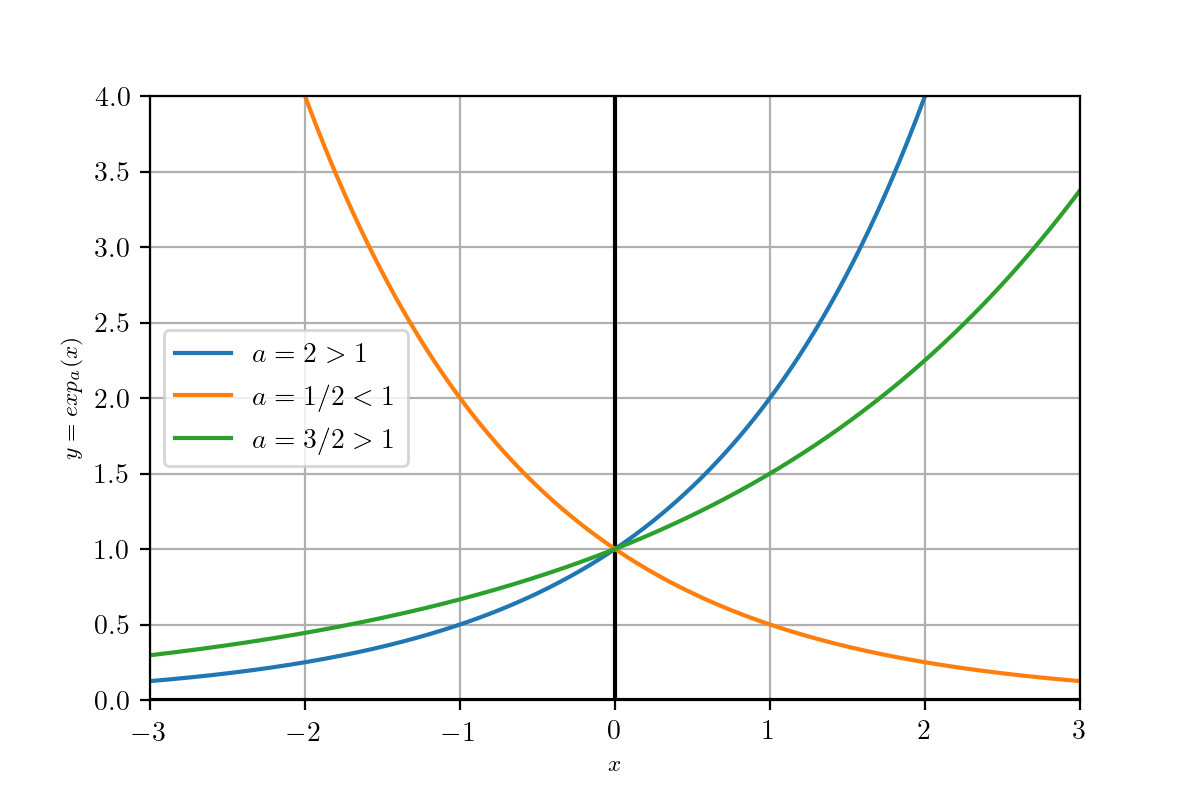
\includegraphics[scale=0.6]{expa.png}
  \caption{Tracé des exponentielles de base quelconque}
  \label{fig:traceexpa}
\end{figure}
%
\section{Puissances}
\label{sec:chap1-puissances}
\subsection{Les fonctions puissances}
\label{subsec:chap1-fonctionspuissances}
\begin{defdef}
  Soit un réel \(\alpha\). On appelle fonction puissance d'exposant \(\alpha\) la fonction
  \begin{equation}
    \fonction{f_{\alpha}}{\Rplusetoile}{\R}{x}{x^{\alpha}=\e^{\alpha \ln x}}.
  \end{equation}
\end{defdef}
%
\begin{prop}
  Soient deux réels \(\alpha\) et \(x\), alors les formules suivantes sont vraies~:
  \begin{gather}
    1^{\alpha}=1; \\
    x^0=1; \\
    \ln x^{\alpha} = \alpha \ln x.
  \end{gather}
\end{prop}
\begin{proof}
  Ce sont des conséquences immédiates de la définition.
\end{proof}
%
\begin{prop}
  Soient deux réels \(\alpha\) et \(\beta\), puis deux réels strictement positifs \(x\) et \(y\). Les formules suivantes sont vraies
  \begin{gather}
    x^{\alpha+\beta}=x^\alpha x^\beta;\\
    (xy)^\alpha = x^\alpha y^\alpha;\\
    (x^\alpha)^\beta=x^{\alpha\beta}.
  \end{gather}
\end{prop}
\begin{proof}
  Soient deux réels \(\alpha\) et \(\beta\), puis deux réels strictement positifs \(x\) et \(y\). Alors
  \begin{gather}
  x^{\alpha+\beta}=\e^{(\alpha+\beta)\ln x}=\e^{\alpha \ln x} \e^{\beta \ln x}=x^\alpha x^\beta;\\
  (xy)^\alpha=\e^{\alpha \ln (xy)}=\e^{\alpha \ln x +\alpha \ln y}=\e^{\alpha \ln x} \e^{\alpha \ln y}=x^\alpha x^\beta ;\\
  (x^\alpha)^\beta=(\e^{\alpha \ln x})^\beta=\e^{\beta \ln(\e^{\alpha \ln x})}=\e^{\beta \alpha \ln x}=x^{\alpha \beta}.
  \end{gather}
\end{proof}

Les fonctions puissances admettent les limites suivantes~:
\begin{equation}
  \begin{cases}
    \alpha=0 & f_0=\tilde{1};\\
    \alpha>0 & \lim\limits_{+\infty}f_\alpha=+\infty \quad \lim\limits_{0^{+}}f_\alpha=0;\\
    \alpha<0 & \lim\limits_{+\infty}f_\alpha=0 \quad \lim\limits_{0^{+}}f_\alpha=+\infty.
  \end{cases}
\end{equation}
\begin{prop}
  Pour tout \(\alpha \in \R\), la fonction \(f_\alpha\) est dérivable sur \(\Rplusetoile\) telle que
  \begin{equation}
    \forall x \in \Rplusetoile \quad f'_\alpha(x)=\alpha x^{\alpha -1}.
  \end{equation}
\end{prop}
\begin{proof}
  La fonction \(f_\alpha\) est dérivable par composition de fonctions qui le sont et pour tout \(x > 0\) on a
  \begin{equation}
    f_\alpha'(x)=\frac{\alpha}{x} \e^{\alpha \ln x}=\frac{\alpha}{x} x^\alpha=\alpha x^{\alpha-1}.
  \end{equation}
\end{proof}

Lorsque \(\alpha \geqslant 0\), les fonctions \(f_\alpha\) peuvent se prolonger en zéro pour obtenir une fonction continue. Deux cas se présentent~:
\begin{itemize}
\item Si \(\alpha>0\) on pose \(\fonction{\tilde{f}_\alpha}{\Rpluss}{\R}{x}{\begin{cases} f_\alpha(x) & x>0 \\ 0 & x=0 \end{cases}}\);
\item Si \(\alpha=0\) on pose \(\fonction{\tilde{f}_0}{\Rpluss}{\R}{x}{1}\).
\end{itemize}
Le prolongement en zéro des fonction puissances s'effectue de cette manière~:
\begin{itemize}
\item Si \(\alpha=0 \quad \tilde{f}_0\) est dérivable et sa dérivée est nulle;
\item Si \(\alpha>1 \quad x^{\alpha-1}\underset{x \to 0^+}{\longrightarrow}0\), le prolongement par continuité \(\tilde{f}_\alpha\) est dérivable en 0 et \(\tilde{f}_\alpha'(0)=0\) La courbe admet une tangente horizontale;
\item Si \(\alpha=1 \quad x^{\alpha-1}\underset{x \to 0^+}{\longrightarrow}1\), le prolongement  \(\tilde{f}_1\) est dérivable en 0 et \(\tilde{f}_1'(0)=1\);
\item Si \(0<\alpha<1 \quad x^{\alpha-1}\underset{x \to 0^+}{\longrightarrow}+\infty \), le prolongement \(\tilde{f}_\alpha\) n'est pas dérivable en zéro et la courbe admet une tangente verticale.
\end{itemize}
%
\begin{figure}
  \centering
  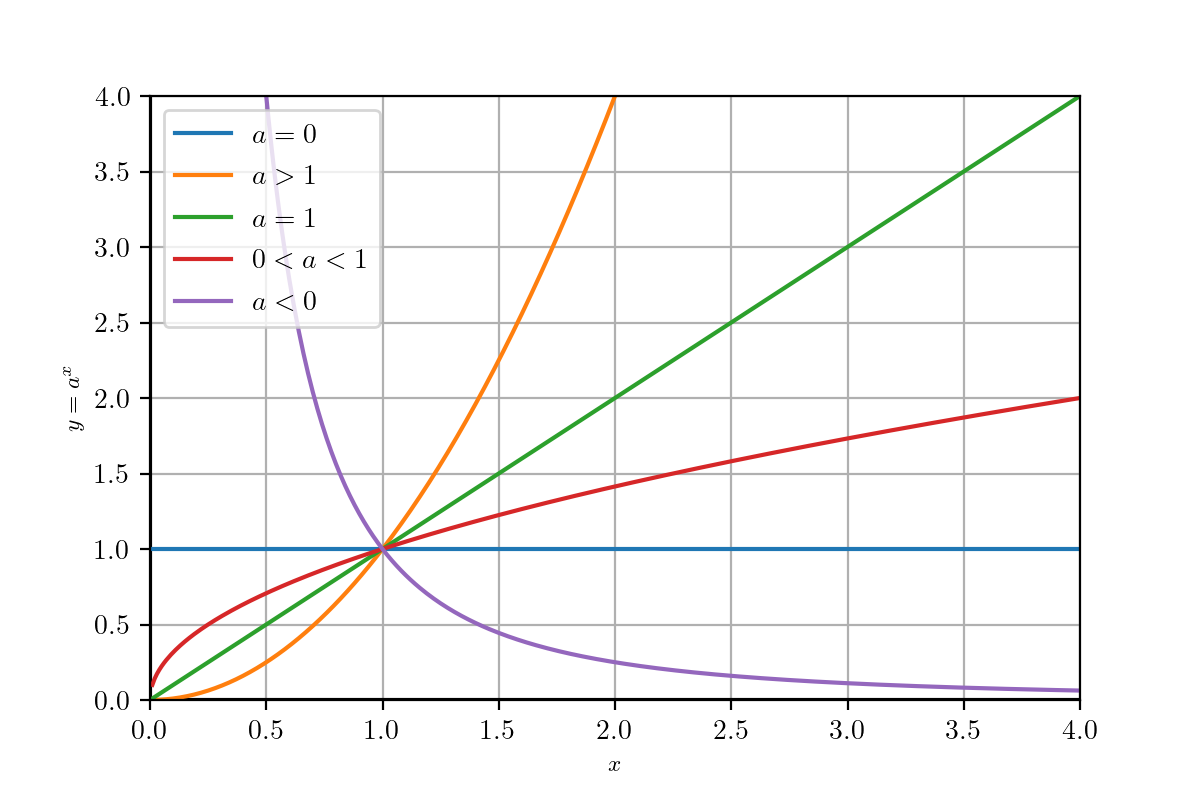
\includegraphics[scale=0.6]{puiss.png}
  \caption{Tracé de quelques fonctions puissance}
  \label{figtracepuissance}
\end{figure}

Si \(\alpha \neq 0\), les fonctions \(f_{\frac{1}{\alpha}}\) et \(f_\alpha\) sont réciproques l'une de l'autre.
%
\subsection{Dérivation des fonctions de la forme exponentielle}
\label{subsec:chap1-derivationdesfonctionsdelaformeexponentielle}
\begin{prop}
  Soient \(I\) un intervalle réel, \(u\) et \(v\) des fonctions dérivables de \(\R^{I}\), alors la fonction \(u^v\) est dérivable.
\end{prop}
\begin{proof}
  Soit un réel \(x\) de \(I\) et soit \(f(x)=\e^{v(x) \ln u(x)}\). La fonction \(f\) est dérivable comme produit et composée de fonctions qui le sont, et
  \begin{align}
    f'(x) &=\left[ v'(x) \ln u(x) + v(x) \frac{u'(x)}{u(x)} \right]\e^{v(x) \ln u(x)} \\
    &= \left[v'(x)u(x)\ln u(x) + v(x) u'(x) \right]u(x)^{v(x)-1}.
  \end{align}
\end{proof}
%
\section{Croissances comparées}
\label{sec:chap1-croissancescomparees}
\begin{theo}
  \begin{equation}
    \lim\limits_{x \to +\infty} \frac{\ln x}{x}=0^+.
  \end{equation}
  Ce qui traduit la \og lenteur \fg{} de croissance du logarithme népérien par rapport à l'identité. On écrira par la suite \(\ln x=o_{+\infty}(x)\).
\end{theo}
\begin{proof}
  Soient deux réels \(x\) et \(t\) supérieurs à 1, alors
  \begin{align}
    \sqrt{t} & \leqslant t \\
    \frac{1}{t} &\leqslant \frac{1}{\sqrt{t}}\\
    0 \leqslant \ln x = \int_{1}^{x} \frac{\diff t}{t} &\leqslant \int_1^x\frac{\diff t}{\sqrt{t}}=2\sqrt{x}-2\\
    0 \leqslant \frac{\ln x}{x} &\leqslant \frac{2}{\sqrt{x}} - \frac{2}{x}.
  \end{align}
  En passant à la limite, et d'après le théorème des gendarmes on obtient la limite en zéro.
\end{proof}
%
\begin{prop}
  \label{prop-chap1:croissancecomparelnpuissance}
  Soient \(\alpha\) et \(\beta\) deux réels strictement positifs, alors
  \begin{equation}
    \lim\limits_{x \to +\infty} \frac{(\ln x)^\alpha}{x^\beta} = 0^+ \quad \lim\limits_{x \to 0^+} x^\beta \abs{\ln x}^\alpha=0^+.
  \end{equation}
  Ce qui veut dire que les puissances \og l'emportent \fg{} toujours devant les logarithmes.
\end{prop}
\begin{proof}
  Soit un réel \(x \geqslant 1\) alors
  \begin{equation}
    \frac{\ln x^\alpha}{x^\beta}=\left(\frac{\alpha}{\beta} \frac{\ln x^{\frac{\beta}{\alpha}}}{x^{\frac{\beta}{\alpha}}} \right)^\alpha.
  \end{equation}
  On a
  \begin{equation}
    x^{\frac{\beta}{\alpha}}\underset{x \to +\infty}{\longrightarrow}+\infty,
  \end{equation}
  donc par composition de limites
  \begin{equation}
    \lim\limits_{x \to \infty} \frac{\ln x^{\frac{\beta}{\alpha}}}{x^{\frac{\beta}{\alpha}}}=0^{+}.
  \end{equation}
  Ainsi
  \begin{equation}
    \frac{\ln x ^\alpha}{x^\beta}=\e^{\alpha \ln \left(\frac{\alpha}{\beta} \frac{\ln x^{\frac{\beta}{\alpha}}}{x^{\frac{\beta}{\alpha}}} \right)} \underset{x \to +\infty}{\longrightarrow}0.
  \end{equation}
  La deuxième limite peut s'obtenir en faisant apparaître \(\frac{1}{x}\)~: soit un réel \(x\) tel que \(0<x<1\), alors
  \begin{equation}
    x^\beta \abs{\ln x}^\alpha=\frac{\abs{-\ln\left(\frac{1}{x}\right)}^\alpha}{\left(\frac{1}{x} \right)^\beta}=\frac{\ln\left(\frac{1}{x}\right)^\alpha}{\left(\frac{1}{x}\right)^\beta}.
  \end{equation}
  Soit en appliquant la première limite ---~puisque \(\frac{1}{x}\underset{x \to 0^+}{\longrightarrow}+\infty\)~--- on obtient le résultat.
\end{proof}
%
\begin{prop}
  Soient \(\alpha\) et \(\beta\) deux réels strictement positifs, alors
  \begin{equation}
    \lim\limits_{x \to + \infty} \frac{\e^{\alpha x}}{x^\beta}=+\infty \quad \lim\limits_{x \to -\infty} \e^{\alpha x} \abs{x}^\beta=0^+.
  \end{equation}
  Ce qui traduit la prépondérance des fonctions exponentielles face aux fonctions puissances.
\end{prop}
%
\begin{proof}
  Soit un réel \(x\) strictement positif. On pose \(y=\e^{x}\) alors
  \begin{equation}
    \frac{\e^{\alpha x}}{x^\beta}=\frac{y^\alpha}{\ln(y)^\beta},
  \end{equation}
  puisque \(\e^{x} \underset{x \to \infty}{\longrightarrow}+\infty\) la proposition~\ref{prop-chap1:croissancecomparelnpuissance} nous permet d'écrire que par composition de limites, la première limite est vraie
  \begin{equation}
    \lim\limits_{x \to + \infty} \frac{\e^{\alpha x}}{x^\beta}=+\infty.
  \end{equation}
  Soit un réel \(x\) strictement négatif, alors
  \begin{equation}
    \e^{\alpha x}\abs{x}^\beta=\frac{(-x)^\beta}{\e^{\alpha(-x)}}.
  \end{equation}
  D'après la première limite
  \begin{equation}
    \lim\limits_{x \to - \infty} \frac{\e^{\alpha (-x)}}{(-x)^\beta}=+\infty.
  \end{equation}
  D'où
  \begin{equation}
    \lim\limits_{x\to -\infty}\frac{(-x)^\beta}{\e^{\alpha (-x)}}=\lim\limits_{x \to -\infty} \e^{\alpha x} \abs{x}^\beta=0^+.
  \end{equation}
\end{proof}
%
\section{Trigonométrie circulaire}
\label{sec:chap1-trigocirc}
On présente un tableau récapitulatif~\ref{tab:fonctiontrigo} des différentes fonctions trigonométriques de base et leurs propriétés. On a tracé les mêmes fonctions sur le cercle trigonométrique de la figure~\ref{fig:cercletrigo}.
\begin{table}[!h]
  \centering
  \begin{tabular}{|c|c|c|c|c|}
    \hline
    Nom & définie sur & parité & T & propriétés \\ \hline
    sinus & \(\R\) & impaire & \(2\pi\) & \(\sin(\pi+x)=-\sin x\) \\
    & & & & \(\sin(\pi-x)=\sin x\) \\ \hline
    cosinus & \(\R\) & paire & \(2\pi\) & \(\cos(\pi+x)=-\cos x\)\\
    & & & & \( \sin(\pi-x)=-\cos x\) \\ \hline
    tangente & \(D_1=\R\setminus\{\frac{\pi}{2}+\pi \Z\}\) & impaire & \(\pi\) & \(\tan x =\frac{\sin x}{\cos x}\) \\ \hline
    cotangente & \(D_2=\R\setminus\{\pi \Z\}\) & paire & \(\pi\) & \(\cot x =\frac{\cos x}{\sin x}\) \\ \hline
  \end{tabular}
  \caption{Fonctions trigonométriques de base}
  \label{tab:fonctiontrigo}
\end{table}

%\begin{figure}
%\centering
%\begin{tikzpicture}
%\draw (0,0) circle (4);
%\draw (180:4) -- (0:4);
%\draw (-90:4) -- (90:4);
%\draw (1,0) arc(0:35:1) node[right, below]{\(\theta\)};
%\draw (0,0) -- (35:4) node[midway, above, sloped]{\(1\)};
%\draw[color=blue] (35:4) -- (0,2.29) node[midway, above, sloped]{\(\cos \theta\)};
%\draw[color=red] (35:4) -- (3.276,0) node[midway, below, sloped]{\(\sin \theta\)};
%%\draw (4,-4) --++ (0,8);
%\draw[color=yellow](35:4) -- (4,2.8);%Pour compléter la tangente
%\draw[color=orange](4,2.8) -- (5.71,4);
%\draw[color=green] (4,0) -- (4,2.8) node[midway, below, sloped]{\(\tan \theta\)};
%\draw[color=pink] (0,4) -- (5.71,4) node[midway, above, sloped]{\(\cot \theta\)};
%\end{tikzpicture}
%\caption{Cercle trigonométrique}
%\label{fig:cercletrigo}
%\end{figure}
\begin{figure}
\centering
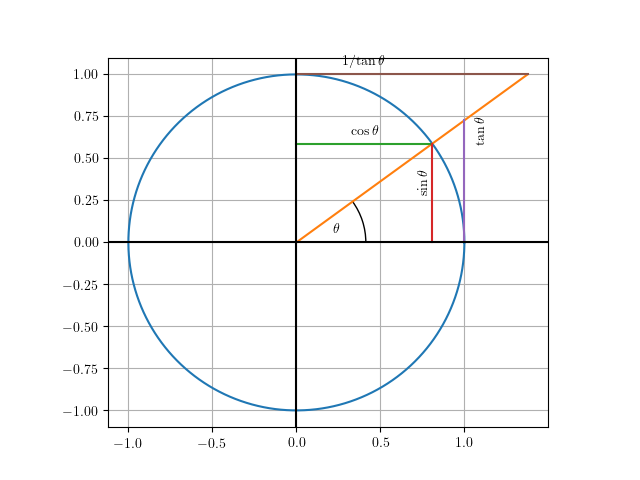
\includegraphics[scale=0.7]{./CercleTrigo.png}
\caption{Cercle trigonométrique}
\label{fig:cercletrigo}
\end{figure}
%
Soit un réel \(x\) et un réel \(y \in D_2\), alors
\begin{gather}
  \cos^2 x+\sin^2 x=1;\\
  \sin \left(\frac{\pi}{2}-x\right)=\cos x=\sin \left(\frac{\pi}{2}+x\right); \\
  \cos \left(\frac{\pi}{2}-x\right)=\sin x=-\cos\left(\frac{\pi}{2}+x\right);\\
  \tan \left(\frac{\pi}{2}-y \right)=\cot y=-\cot \left(\frac{\pi}{2}+y\right).
\end{gather}
%
\begin{figure}
  \centering
  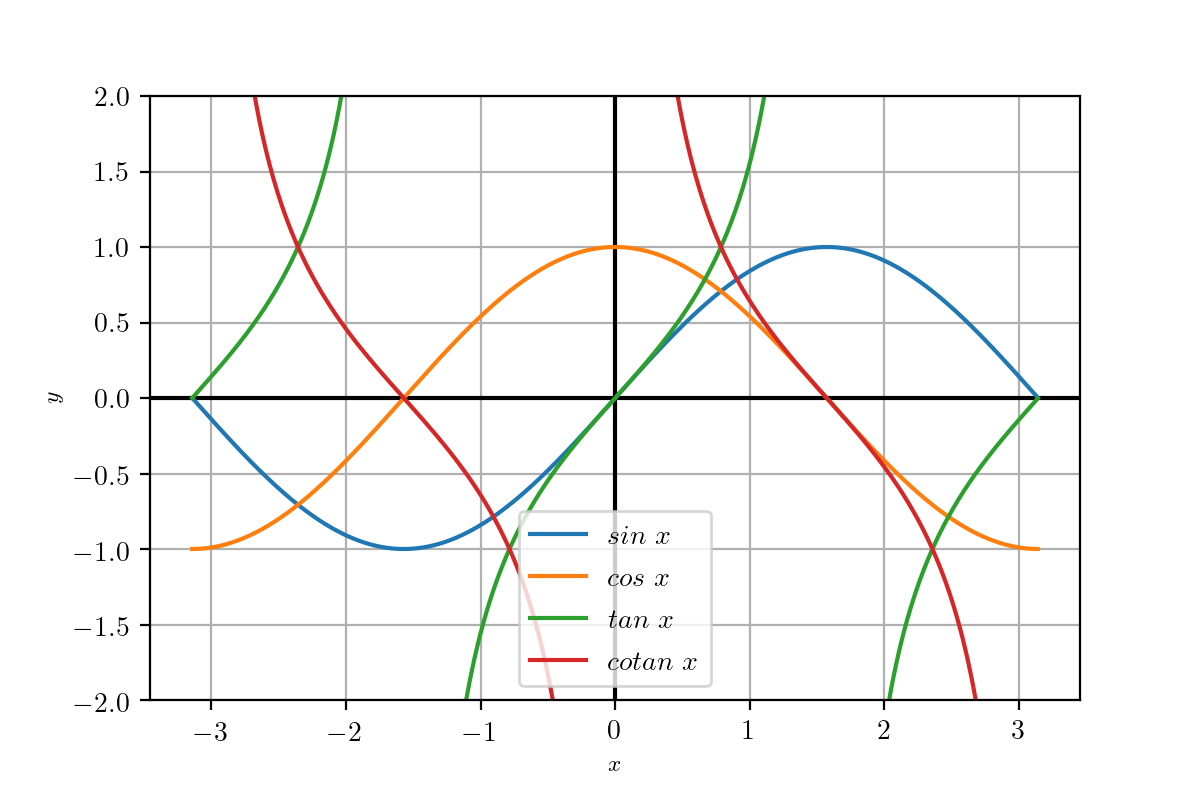
\includegraphics[scale=0.6]{trig.png}
  \caption[Tracé de quelques fonctions trigonométriques]{Tracé de quelques fonctions trigonométriques. En rouge sinus, en bleu cosinus, en vert tangente et en rose cotangente}
  \label{fig:tracetrigo}
\end{figure}
%
\renewcommand{\arraystretch}{2.2}
\begin{table}
  \centering
  \begin{tabular}{|c|c|c|c|c|c|}
    \hline
    \(\displaystyle x\)& \(\displaystyle 0\)&\(\displaystyle \frac{\pi}{6}\)&\(\displaystyle \frac{\pi}{4}\)&\(\displaystyle \frac{\pi}{3}\)&\(\displaystyle \frac{\pi}{2}\)\\ \hline
    \(\displaystyle \sin x\) &\(\displaystyle  0\) &\(\displaystyle  \frac{1}{2}\) &\(\displaystyle  \frac{\sqrt{2}}{2}\) & \(\displaystyle \frac{\sqrt{3}}{2}\) &\(\displaystyle  1 \)\\ \hline
    \(\displaystyle \cos x\) &\(\displaystyle  1 \)&\(\displaystyle \frac{\sqrt{3}}{2}\) & \(\displaystyle \frac{\sqrt{2}}{2}\) & \(\displaystyle \frac{1}{2}\) & \(\displaystyle 0\) \\ \hline
    \(\displaystyle \tan x\) & \(\displaystyle  0 \)&\(\displaystyle \frac{1}{\sqrt{3}}\) & \(\displaystyle 1\) & \(\displaystyle \sqrt{3}\) & \(\displaystyle \infty\) \\ \hline
    \(\displaystyle \cot x\) & \(\displaystyle \infty\) & \(\displaystyle \sqrt{3}\) &\(\displaystyle  1\) & \(\displaystyle \frac{1}{\sqrt{3}}\) &\(\displaystyle  0\)\\ \hline
  \end{tabular}
  \caption{Valeurs particulières des fonctions trigonométriques}
  \label{tab:valeurpart}
\end{table}
\renewcommand{\arraystretch}{1}
\paragraph{Dérivées}
Les fonctions sinus, cosinus, tangente et cotangente sont dérivables sur leurs ensembles de définition, et on a:
\begin{gather}
\forall x \in \R \quad \sin'x=\cos x \ \cos'x=-\sin x; \\
\forall x \in D_1 \quad \tan'x=\frac{1}{\cos^2 x}=1+\tan^2 x; \\
\forall x \in D_2 \quad \cot'x=\frac{-1}{\sin^2 x}=-1-\cot^2 x.
\end{gather}
\begin{prop}
  Les fonctions trigonométriques vérifient les égalités suivantes~:
  \begin{gather}
    \forall x, y \in \R \quad \cos x = \cos y \iff \exists k \in \Z \ x=\pm y + 2k\pi;\\
    \forall x, y \in \R \quad \sin x = \sin y \iff \begin{cases} \exists k \in \Z & x = y + 2 k \pi \\ \exists k \in \Z & x = \pi - y + 2 k \pi\end{cases}; \\
    \forall x, y \in D_1 \quad \tan x = \tan y \iff \exists k \in \Z \ x = y + k \pi;\\
    \forall x, y \in D_2 \quad \cot x = \cot y \iff \exists k \in \Z \ x = y + k \pi.
  \end{gather}
\end{prop}

\section{Fonctions circulaires réciproque}
\label{sec:chap1-fonctionscircréciproques}
\subsection{Fonction arcsinus}
\label{subsec:chap1-fonctionarcsinus}
\begin{defdef}
  La fonction \(\fonction{\sin}{\intervalleff{-\frac{\pi}{2}}{\frac{\pi}{2}}}{\intervalleff{-1}{1}}{x}{\sin x}\) est une bijection~\footnote{parce qu'elle est continue, strictement croissante telle que \(\sin -\frac{\pi}{2}=-1\)  et \(\sin \frac{\pi}{2}=1\)} et cette bijection admet une réciproque appelée arcsinus notée \(\arcsin\).
\end{defdef}
%
\begin{prop}
  \begin{equation}
    \forall x \in \intervalleff{-\frac{\pi}{2}}{\frac{\pi}{2}} \forall y \in \intervalleff{-1}{1} \quad y = \sin x \iff x = \arcsin y;
  \end{equation}
  et
  \begin{gather}
    \sin(\arcsin y)) = y, \\
    \arcsin(\sin x) = x.
  \end{gather}
\end{prop}
\begin{proof}
  C'est une conséquence de la définition de \(\arcsin\).
\end{proof}
\emph{Remarque~:} La formule \(\arcsin(\sin x) = x\) n'est valable que dans \(\intervalleff{-\frac{\pi}{2}}{\frac{\pi}{2}}\) et la deuxième dans \(\intervalleff{-1}{1}\).
%
\begin{prop}
  La fonction \(\arcsin\) est impaire et strictement croissante.
\end{prop}
\begin{proof}
  La fonction \(\arcsin\) est croissante par construction car sa réciproque est strictement croissante. Ensuite, l'intervalle \(\intervalleff{-1}{1}\) est centré en 0 et puisque sinus est impaire on a
  \begin{equation}
    \forall y \in \intervalleff{-1}{1} \quad \sin (\arcsin -y)=-y=-\sin(\arcsin y)=\sin (-\arcsin y).
  \end{equation}
  En appliquant la fonction \(\arcsin\)~\footnote{qui est bijective} à chaque membre, on trouve que la fonction \(\arcsin\) est impaire.
\end{proof}
%
\begin{prop}
  La fonction arcsinus est dérivable sur \(\intervalleoo{-1}{1}\) et
  \begin{equation}
    \forall y \in \intervalleoo{-1}{1} \quad \arcsin'y = \frac{1}{\sqrt{1-y^2}}.
  \end{equation}
\end{prop}
\begin{proof}
  La fonction sinus est dérivable sur \(\intervalleff{-\frac{\pi}{2}}{\frac{\pi}{2}}\) telle que \(\sin'=\cos\). Si \(y=\pm 1\) alors \(\cos(\arcsin y)=0\) et donc arcsinus n'est pas dérivable. De plus la courbe représentative admet des tangentes verticales en \(-1\) et \(1\). Si \(y \in \intervalleoo{-1}{1}\), alors \(\cos(\arcsin y) \neq 0\), arcsinus et donc dérivable en \(y\) et
  \begin{equation}
    \arcsin' y = \frac{1}{\cos( \arcsin y)}=\frac{1}{\sqrt{1-\sin^2(\arcsin y)}}=\frac{1}{\sqrt{1-y^2}}.
  \end{equation}
\end{proof}
\begin{figure}
  \centering
  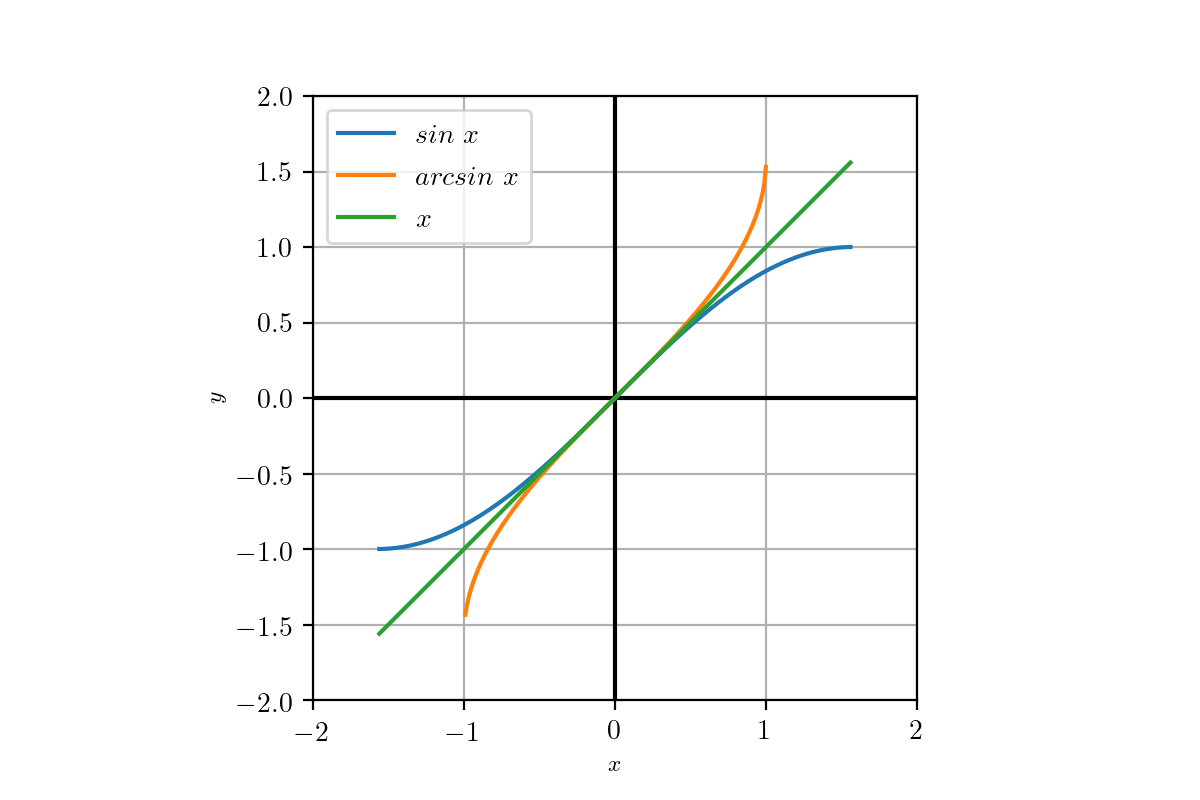
\includegraphics[scale=0.7]{arcsin.png}
  \caption{Tracé de arcsinus}
  \label{fig:tracearcsinus}
\end{figure}
%
\subsection{Fonction arccosinus}
\label{subsec:chap1-fonctionarccos}
\begin{defdef}
  La fonction \(\fonction{\cos}{\intervalleff{0}{\pi}}{\intervalleff{-1}{1}}{x}{\cos x}\) est une bijection~\footnote{parce qu'elle est continue, strictement décroissante telle que \(\cos 0=1\) et \(\cos \pi=-1\).} et cette bijection admet une réciproque appelée arccosinus notée \(\arccos\).
\end{defdef}
%
\begin{prop}
  \begin{equation}
    \forall x \in \intervalleff{0}{\pi} \forall y \in \intervalleff{-1}{1} \quad y = \cos x \iff x = \arccos y;
  \end{equation}
  et
  \begin{gather}
    \cos(\arccos y) = y, \\
    \arccos(\cos x) = x.
  \end{gather}
\end{prop}
\begin{proof}
  C'est une conséquence de la définition de la fonction \(\arccos\).
\end{proof}
%
\emph{Remarque~:} La première formule n'est valable que dans l'intervalle \(\intervalleff{0}{\pi}\) et la deuxième dans l'intervalle \(\intervalleff{-1}{1}\).
\begin{prop}
  La fonction \(\arccos\) est strictement décroissante.
\end{prop}
\begin{proof}
  La fonction \(\arccos\) est décroissante par construction.
\end{proof}
%
\begin{prop}
  La fonction arcsinus est dérivable sur \(\intervalleoo{-1}{1}\) et
  \begin{equation}
    \forall y \in \intervalleoo{-1}{1} \quad \arccos'y = -\frac{1}{\sqrt{1-y^2}}.
  \end{equation}
\end{prop}
\begin{proof}
  La fonction cosinus est dérivable sur l'intervalle \(\intervalleff{0}{\pi}\) telle que \(\cos'=-\sin\). Si \(y=\pm 1\) alors \(-\sin(\arccos(y))=0\)  et donc arccosinus n'est pas dérivable. De plus la courbe représentative admet des tangentes verticales en \(-1\) et \(1\). Si \(y \in \intervalleoo{-1}{1}\), alors \(-\sin(\arccos y) \neq 0\), arccosinus et donc dérivable en \(y\) et
  \begin{equation}
    \arccos' y = \frac{1}{-\sin( \arccos y)}=\frac{-1}{\sqrt{1-\cos^2(\arccos y)}}=\frac{-1}{\sqrt{1-y^2}}.
  \end{equation}
\end{proof}
%
\begin{figure}
  \centering
  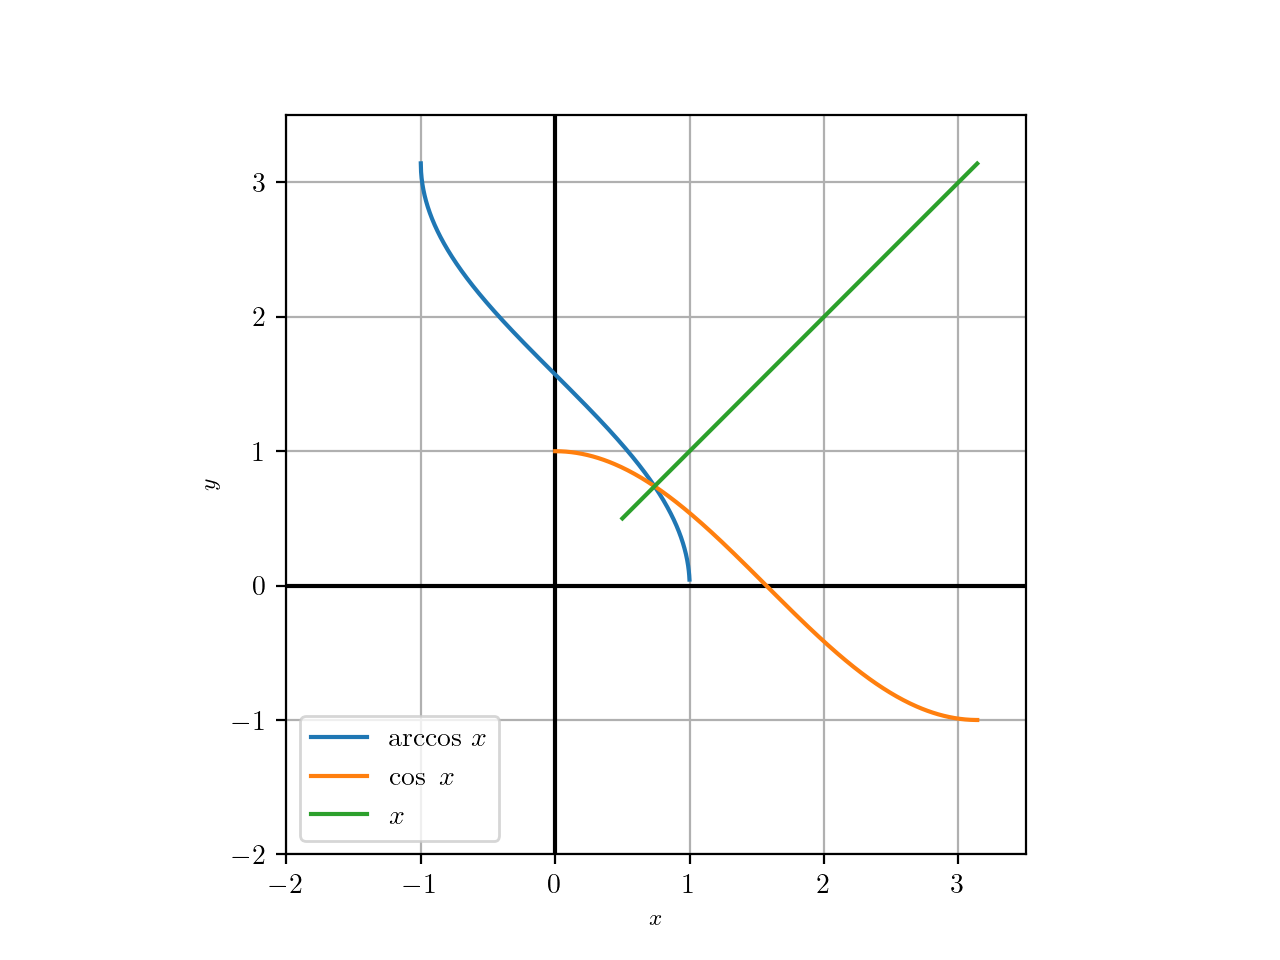
\includegraphics[scale=0.7]{arccos.png}
  \caption{Tracé de arccosinus}
  \label{fig:tracearccosinus}
\end{figure}
%
\begin{prop}
  Soit un réel \(x\) de \(\intervalleff{-1}{1}\), alors on a
  \begin{gather}
    \cos( \arcsin x)=\sin( \arccos x)=\sqrt{1-x^2}; \\
    \arccos x + \arcsin x = \frac{\pi}{2};\\
    \arccos(-x) = \pi - \arccos x.
  \end{gather}
\end{prop}
\begin{proof}
  \begin{itemize}
  \item puisque \(\arcsin x \in \intervalleff{-\frac{\pi}{2}}{\frac{\pi}{2}}\) alors
    \begin{equation}
      \cos( \arcsin x)=\sqrt{1- \sin^2(\arcsin x)}=\sqrt{1-x^2} \geqslant 0
    \end{equation}
    On fait le même raisonnement avec \(\arccos x\).
  \item On sait aussi que
    \begin{equation}
      \cos( \arccos x) = x = \sin( \arcsin x)=\cos \left( \frac{\pi}{2} - \arcsin x \right),
    \end{equation}
    et puisque \(\cos\) est bijective sur \(\intervalleff{0}{\pi}\), on a égalité.
  \item De la même manière
    \begin{equation}
      \cos( \arccos -x)=-x=-\cos( \arccos x)=\cos(\pi - \arccos x),
    \end{equation}
    et comme cosinus est bijectif dans \(\intervalleff{0}{\pi}\), on en déduit l'égalité.
  \end{itemize}
\end{proof}
%
\subsection{Fonction arctangente}
\label{subsec:chap1-fonctionarctangente}
\begin{defdef}
  La restriction de la fonction tangente à l'intervalle \(\intervalleoo{-\frac{\pi}{2}}{\frac{\pi}{2}}\) est une bijection~\footnote{Idem}, sa réciproque est la fonction arctangente notée \(\arctan\).
\end{defdef}
\begin{prop}
  Soit un réel \(x\) quelconque et un réel \(y\) non nul. Alors
  \begin{gather}
    \cos(\arctan x)=\frac{1}{\sqrt{1+x^2}};\\
    \sin(\arctan x)=\frac{x}{\sqrt{1+x^2}};\\
    \arctan y + \arctan \frac{1}{y} = \sgn(y) \frac{\pi}{2}.
  \end{gather}
\end{prop}
\begin{proof}
  Soit un réel \(x\) quelconque et un réel \(y\) non nul, alors
  \begin{itemize}
  \item puisque \(-\frac{\pi}{2} < \arctan x < \frac{\pi}{2}\) alors \(\cos(\arctan x)>0\) donc
    \begin{equation}
      \cos(\arctan x)=\sqrt{\cos^2(\arctan x)}=\sqrt{\frac{1}{1+\tan^2(\arctan x)}}=\frac{1}{\sqrt{1+x^2}};
    \end{equation}
  \item de la même manière on a
    \begin{equation}
      \cos(\arctan x)=\sin( \arctan x) \tan(\arctan x) = \frac{x}{\sqrt{1+x^2}};
    \end{equation}
  \item soit la fonction \(\fonction{f}{\Rplusetoile}{\R}{y}{\arctan y + \arctan \frac{1}{y}}\) dérivable et pour tout réel \(y\) positif, on a
    \begin{equation}
      f'(y)=\frac{1}{1+y^2} - \frac{1}{y^2} \cdot \frac{1}{1+\frac{1}{y^2}}=0.
    \end{equation}
    La fonction \(f\) est donc constante et en \(y=1\) on a \(f(1)=\frac{\pi}{2}=f(y)\). Si \(y\) est strictement négatif, alors comme \(\arctan\) est impaire, on a \(f(y)=-\frac{\pi}{2}\).
\end{itemize}
\end{proof}
%
\begin{figure}
  \centering
  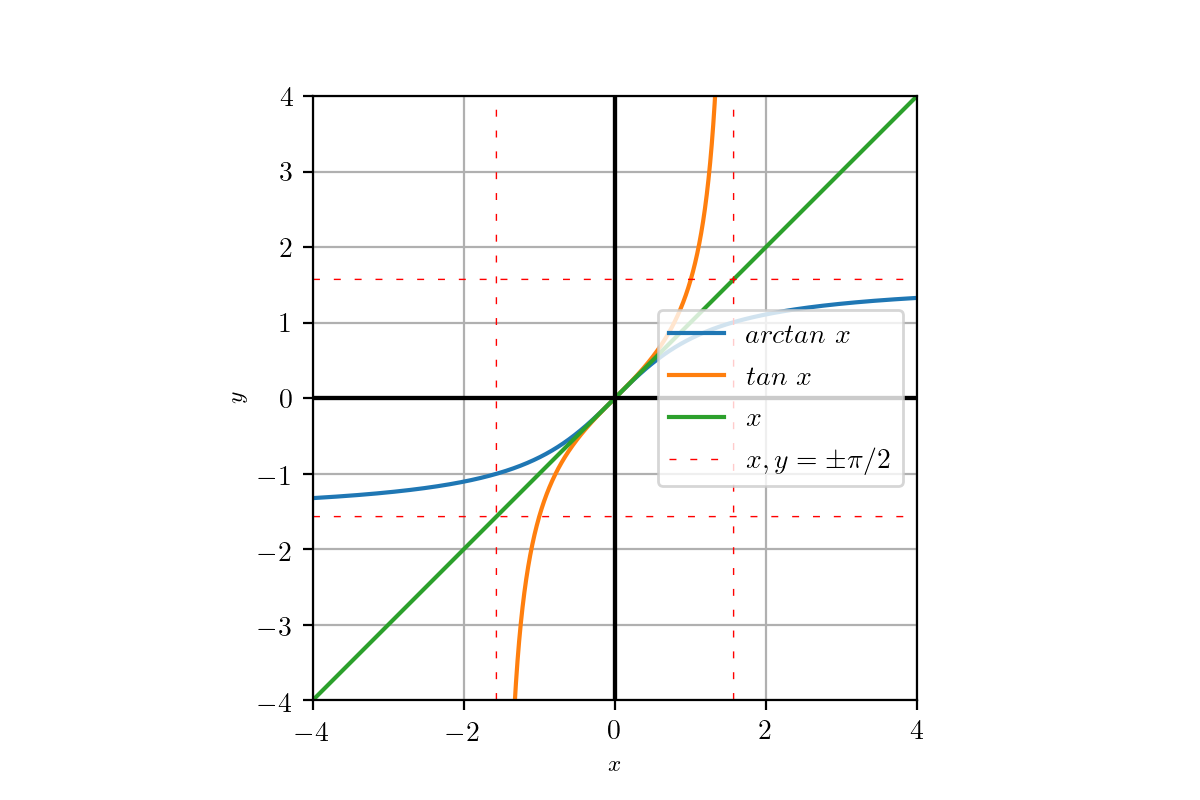
\includegraphics[scale=0.7]{arctan.png}
  \caption{Tracé de arctangente et de ses asymptotes}
  \label{fig:tracearctangente}
\end{figure}
%
\begin{theo}
  \label{chap1-theo:thetasin}
  Soient des réels \(x\) et \(y\) tels que \(x^2+y^2=1\), alors il existe un unique réel \(\theta\) dans \(\intervalleof{-\pi}{\pi}\) tel que \(x=\cos \theta\) et \(y=\sin \theta\).
\end{theo}
\begin{proof}[Existence]
  On sait que \(x^2=1-y^2\) avec \(x^2 \in \intervalleff{0}{1}\) donc \(x \in \intervalleff{-1}{1}\). On peut donc définir un \(\theta_0=\arccos x \in \intervalleff{0}{\pi}\) tel que \(x=\cos \theta_0\). Ainsi \(y^2=1-x^2=\sin^2 \theta_0\). Puisque \(\theta_0 \in \intervalleff{0}{\pi}\) on a \(\sin \theta_0>0\) alors \(\abs{y}=\sin \theta_0\).
Si \(y \geqslant 0\) et comme \(\theta_0 \in \intervalleff{0}{\pi}\), alors \(\theta=\theta_0\) est le bon réel.

Mais si \(y<0\), alors on prend l'opposé \(\theta=-\theta_0 \in \intervalleof{-\pi}{0}\).

On a bien montré l'existence d'un réel \(\theta \in \intervalleof{-\pi}{\pi}\) tel que \(x=\cos \theta\) et \(y=\sin \theta\).
\end{proof}
\begin{proof}[Unicité]
  Supposons qu'il existe deux réel \(\theta\) et \(\theta'\) tels que
  \begin{equation}
    \begin{cases} x=\cos \theta = \cos \theta' \\ y=\sin \theta = \sin \theta' \end{cases},
  \end{equation}
  alors \(x=\cos \abs{\theta}=\cos \abs{\theta'}\) puisque la fonction cosinus est paire. Les réels \(\abs{\theta}\) et \(\abs{\theta'}\) sont dans \(\intervalleff{0}{\pi}\). La restriction de cosinus à \(\intervalleff{0}{\pi}\) est bijective, on en déduit que \(\abs{\theta}=\abs{\theta'}\). Deux cas se présentent~:
  \begin{itemize}
  \item Soit \(\theta'=\theta\);
  \item Soit \(\theta'=-\theta\) et alors \(\sin \theta = \sin \theta' = -\sin \theta\) donc \(\sin \theta = 0\) ainsi, \(\theta = 0\) ou \(\theta = \pi\). Comme \(\theta'=-\theta \in \intervalleof{-\pi}{\pi}\) on a forcément \(\theta = 0 = \theta'\).
\end{itemize}
\end{proof}
%
\section{Trigonométrie hyperbolique}
\label{sec:chap1-trigohyper}
\subsection{Fonctions sinus et cosinus hyperbolique}
\label{subsec:chap1-sinushetcosh}
\begin{defdef}
  On définit les applications de \(\R\) dans \(\R\), appelées respectivement sinus et cosinus hyperbolique, notée \(\hsin\) et \(\hcos\), par
  \begin{gather}
    \forall x \in \R \quad \hsin x = \frac{\e^x - \e^{-x}}{2}, \\
    \forall x \in \R \quad \hcos x = \frac{\e^x + \e^{-x}}{2}.
  \end{gather}
\end{defdef}
%
\begin{prop}
  La fonction sinus hyperbolique est impaire et cosinus hyperbolique est paire. Les fonctions sinus hyperbolique et cosinus hyperbolique sont dérivables sur \(\R\) avec \(\hsin'=\hcos\) et \(\hcos'=\hsin\).
\end{prop}
\begin{proof}
  \(\R\) est centré en \(0\) et ---~grâce aux calculs~--- \(\hsin(-x)=-\hsin x\) et \(\hcos(-x)=\hcos x\). La fonction exponentielle est dérivable sur \(\R\), donc \(\hsin\) et \(\hcos\) sont dérivables et les calculs donnent bien la formule.
\end{proof}
%
\begin{prop} Soit un réel \(x\), alors
\begin{gather}
  \hcos x + \hsin x = \e^x, \\
  \hcos x - \hsin x = \e^{-x}, \\
  \hcos^2 x - \hsin^2 x = 1.
\end{gather}
\end{prop}
\begin{proof}
  Ces formules sont des conséquences de la définition.
\end{proof}
%
\begin{figure}
  \centering
  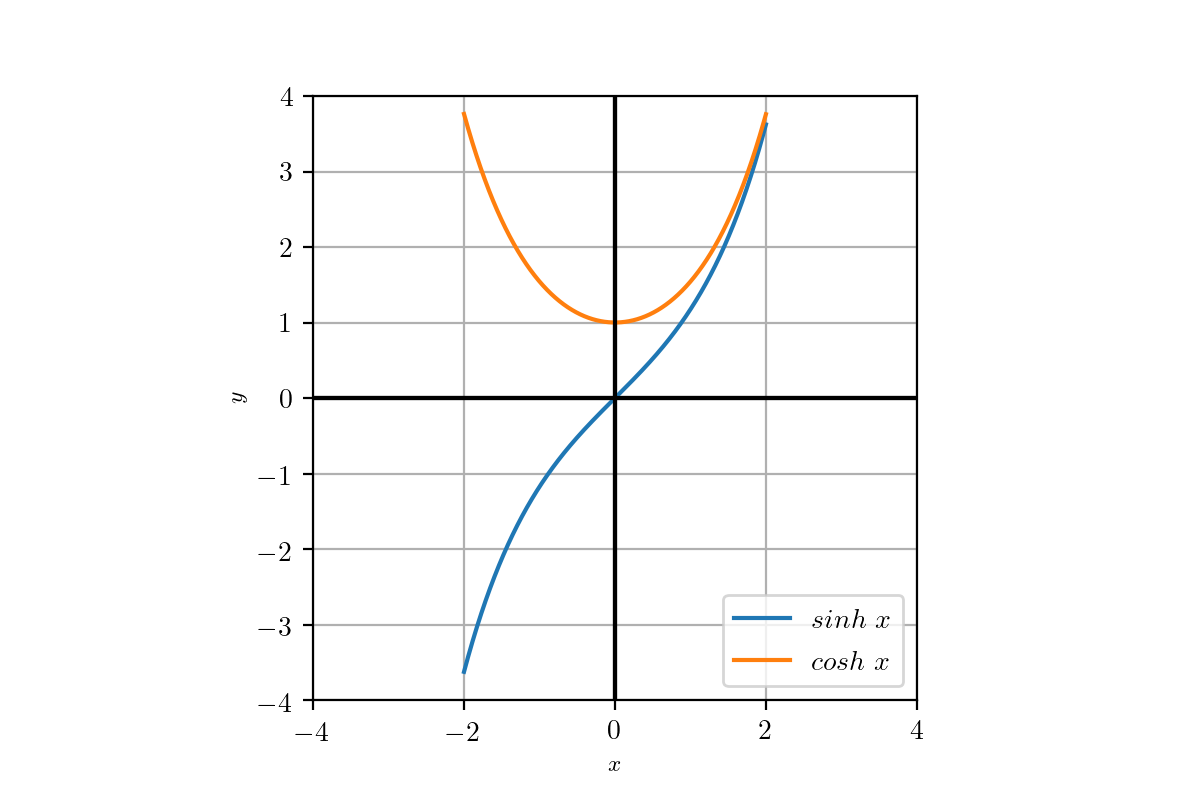
\includegraphics[scale=0.7]{trigh.png}
  \caption{Tracé de fonctions hyperbolique \(\hsin\) et \(\hcos\)}
  \label{fig:tracesinhcosh}
\end{figure}
%
Les fonctions \(\hsin\) et \(\hcos\) permettent de paramétrer l'hyperbole \(\mathcal{H}\) d'équation~: \(\frac{x^2}{a^2} - \frac{y^2}{b^2}=1\)  par \(\begin{cases} x(t)=a \epsilon \hcos t \\ y(t)=b \epsilon \hsin t\end{cases} \epsilon \in \intervalleff{-1}{1}\), d'où le nom de ces fonctions.
%
\subsection{Fonctions tangente et cotangente hyperbolique}
\label{subsec:chap1-tanhetcotanh}
\begin{defdef}
  On définit la tangente hyperbolique, noté \(\htan\), et la cotangente hyperbolique, notée \(\hcotan\), comme
  \begin{gather}
    \forall x \in \R \quad \htan(x)=\frac{\hsin x}{\hcos x}=\frac{\e^x - \e^{-x}}{\e^x+\e^{-x}}, \\
    \forall x \in \R^* \quad \hcotan(x)=\frac{\hcos x}{\hsin x}=\frac{\e^x + \e^{-x}}{\e^x-\e^{-x}}.
  \end{gather}
\end{defdef}
%
\begin{prop}
  Les fonctions tangente et cotangente hyperbolique sont impaires. Elles sont dérivables sur leurs ensembles de définition respectifs et on a
  \begin{equation}
    \forall x \in \R \quad \htan' x = 1-\htan^2 x = \frac{1}{\hcos^2 x}
  \end{equation}
  et
  \begin{equation}
    \forall y \in \Rplusetoile \quad \hcotan' x=1-\hcotan^2 x=-\frac{1}{\hsin^2 x}.
  \end{equation}
\end{prop}
\begin{proof}
  \(\R\) est centré en zéro et on vérifie que
  \begin{gather}
    \htan(-x)=-\htan x, \\
    \hcotan(-x) = -\hcotan x.
  \end{gather}
  Ensuite puisque \(\hsin\) et \(\hcos\) sont dérivables sur \(\R\) et puisque \(\hcos\) ne s'annule pas sur \(\R\), on a pour tout réel \(x\)
  \begin{equation}
    \htan' x = \frac{\hcos^2 x - \hsin^2 x}{\hcos^2 x},
  \end{equation}
  qui nous donne la formule. De la même manière \(\sinh\) ne s'annule qu'en \(x=0\) donc pour \(x\) non nul, on a la formule
  \begin{equation}
    \hcotan' x = \frac{\hsin^2 x - \hcos^2 x}{\hsin^2 x},
  \end{equation}
  qui nous donne aussi la formule.
\end{proof}
La fonction tangente hyperbolique est strictement croissante et la cotangente décroît sur \(\Rmoinsetoile\) et sur \(\Rplusetoile\).
%
\begin{figure}
  \centering
  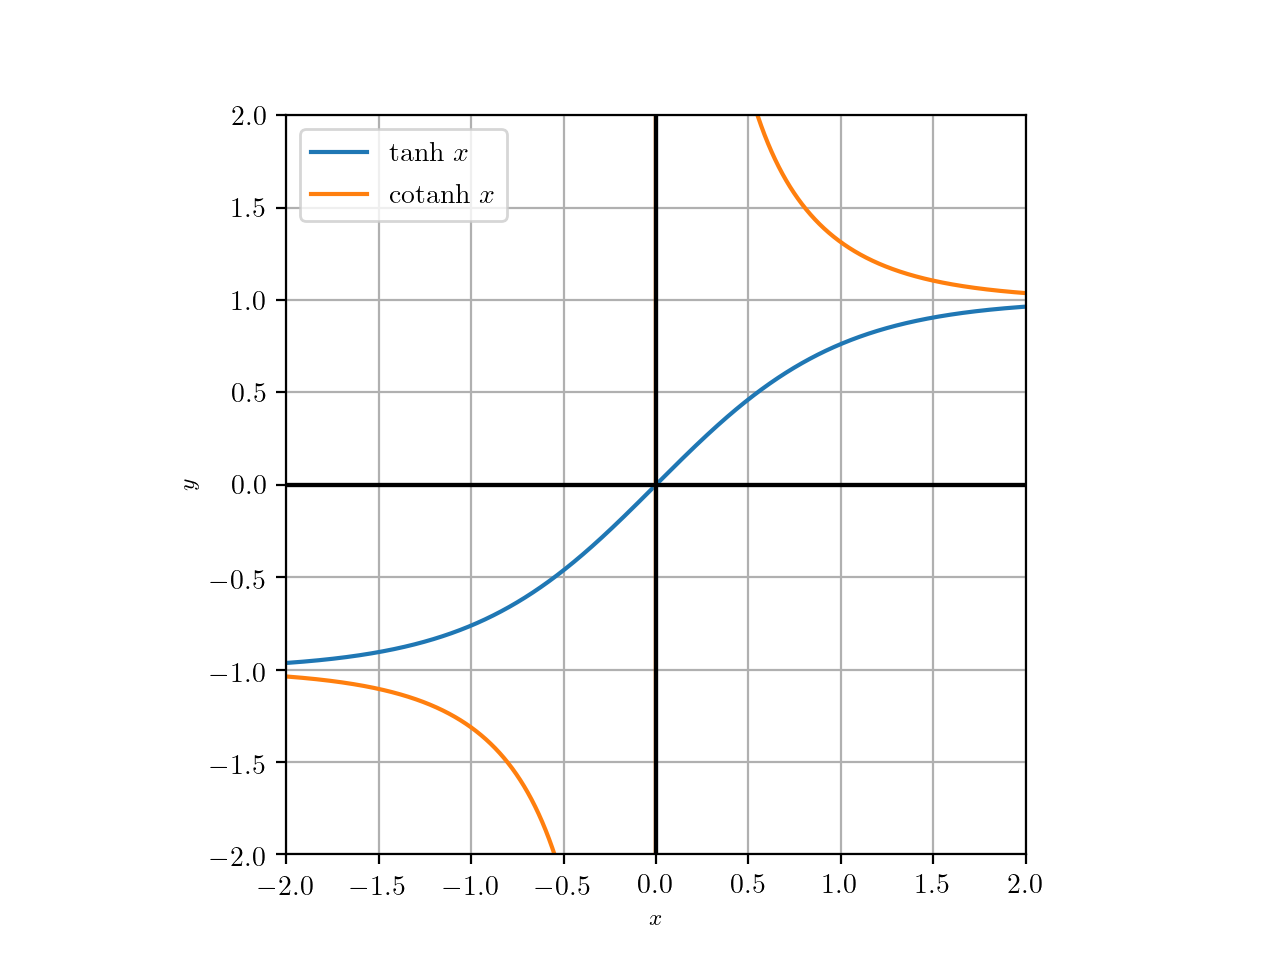
\includegraphics[scale=0.7]{tanh.png}
  \caption{Tracé de fonctions hyperbolique \(\htan\) et \(\hcotan\)}
  \label{fig:tracetanhcoth}
\end{figure}
%
\subsection{Formulaire de trigonométrie hyperbolique}
\label{subsec:chap1-formulairetrigohyp}
En théorie la seule formule exigible est \(\hcos^2-\hsin^2=1\) mais les autres existent, elles peuvent se retrouver à partir du formulaire de trigonométrie circulaire en remplaçant \(\cos\) par \(\hcos\) et \(\sin\) par \(\ii \hsin\).
%
\section{Fonctions hyperboliques réciproques}
\label{sec:chap1-fonctionshyprec}
\subsection{Fonction argument sinus hyperbolique}
\label{subsec:chap1-fonctionargsinh}
\begin{defdef}
  La fonction sinus hyperbolique est une bijection de \(\R\) sur lui-même et admet une réciproque appelée argument sinus hyperbolique notée \(\argsh\).
\end{defdef}
%
\begin{prop}
  \begin{equation}
    \forall x, y \in \R \quad y=\hsin x \iff x=\argsh y.
  \end{equation}
\end{prop}
%
\begin{prop}
La fonction \(\argsh\) est impaire et strictement croissante.
\end{prop}
\begin{proof}
  Soit un réel \(x\), alors
  \begin{equation}
    x=\hsin (\argsh x)=-\hsin(-\argsh x),
  \end{equation}
  donc
  \begin{equation}
    -x=\hsin(\argsh -x)=\hsin(-\argsh x).
  \end{equation}
  Comme la fonction sinus hyperbolique est bijective, on a bien l'égalité
  \begin{equation}
    \argsh(-x)=-\argsh x,
  \end{equation}
  et comme \(\R\) est centré en zéro, alors \(\argsh\) est impaire.
\end{proof}
%
\begin{prop}
  La fonction argument sinus hyperbolique est dérivable sur \(\R\) et pour tout réel \(x\), on a
  \begin{equation}
    \argsh' x= \frac{1}{\sqrt{1+x^2}}.
  \end{equation}
\end{prop}
\begin{proof}
  La fonction sinus hyperbolique est dérivable sur \(\R\) et
  \begin{equation}
    \forall y \in \R \quad \hsin' (\argsh y)=\hcos(\argsh y)>0,
  \end{equation}
  donc la fonction argument sinus hyperbolique est dérivable en \(y\) et
  \begin{equation}
    \argsh' y =\frac{1}{\hcos( \argsh y)}=\frac{1}{\sqrt{1+\hsin^2(\argsh y)}}=\frac{1}{\sqrt{1+y^2}}.
  \end{equation}
\end{proof}
%
\begin{prop}[Expression logarithmique]
La fonction argument sinus hyperbolique peut s'exprimer ainsi
 \begin{equation}
   \forall x \in \R \quad \argsh x = \ln(x+\sqrt{1+x^2}).
 \end{equation}
\end{prop}
\begin{proof}
  Soient deux réels \(x\) et \(y\) tels que \(y=\argsh x\) alors \(x=\frac{\e^y - \e^{-y}}{2}\). C'est-à-dire
  \begin{equation}
    \e^y - \e^{-y} -2x=0,
  \end{equation}
  soit
  \begin{equation}
    \e^{2y}-1-2x\e^{y}=0.
  \end{equation}
  Les solutions réelles de l'équation \(Y^2-2xY-1=0\) sont \(x-\sqrt{x^2+1}<0\) et \(x+\sqrt{x^2+1}\) et donc \(\e^y=x+\sqrt{x^2+1}\) soit pour finir l'expression logarithmique
  \begin{equation}
    \argsh x = y = \ln(x+\sqrt{x^2+1}).
  \end{equation}
\end{proof}
%
\begin{figure}
  \centering
  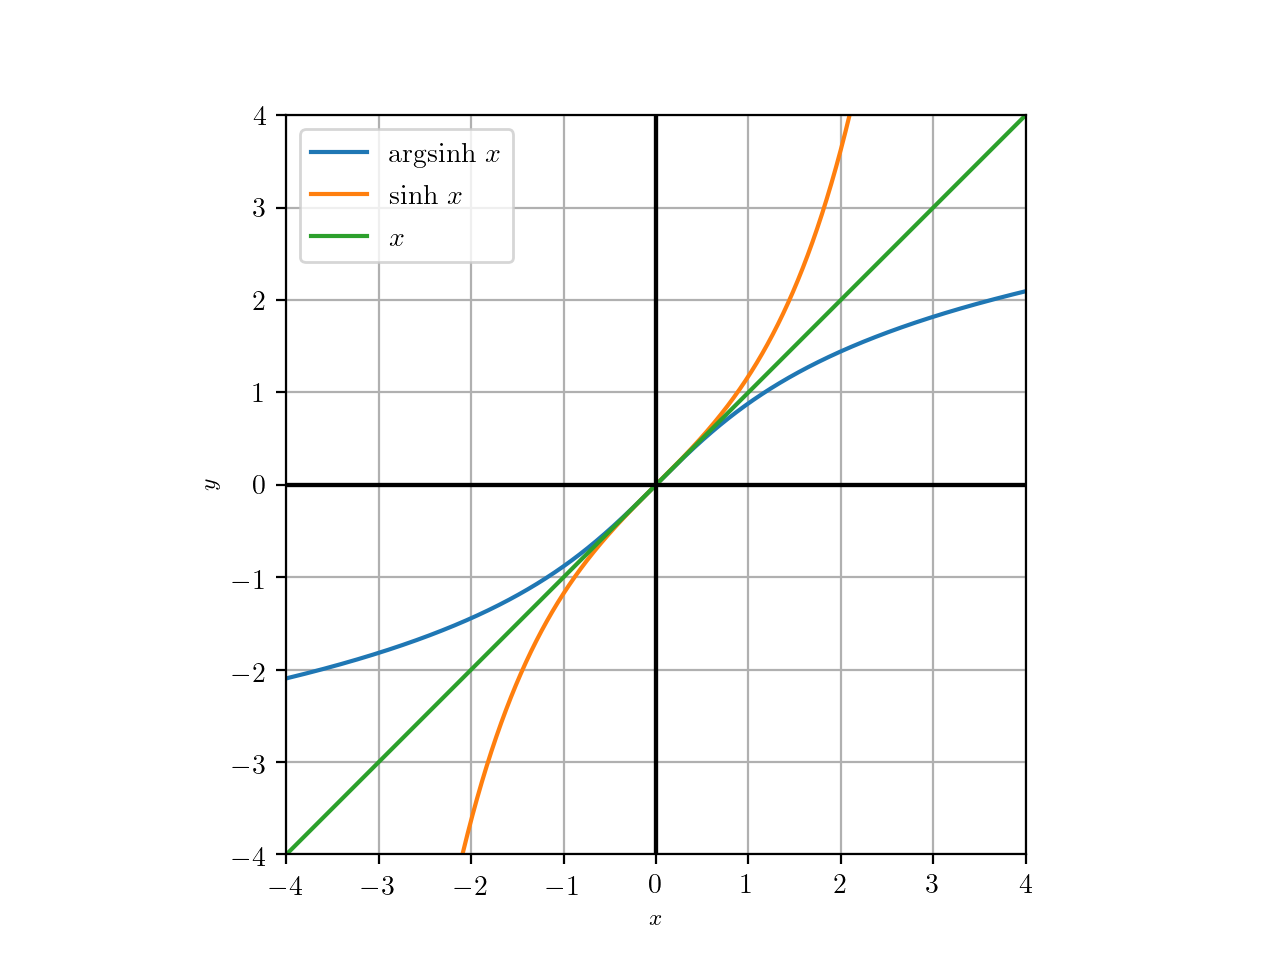
\includegraphics[scale=0.7]{argsinh.png}
  \caption{Tracé de fonctions hyperbolique \(\hsin\) et \(\argsh\)}
  \label{fig:tracesinhargsh}
\end{figure}
%
\subsection{Fonction argument cosinus hyperbolique}
\label{subsec:chap1-fonctionargcosh}
\begin{defdef}
  La fonction cosinus hyperbolique induit une bijection de \(\Rplus\) sur \(\intervallefo{1}{+\infty}\) qui admet une réciproque appelée argument cosinus hyperbolique et notée \(\argch\).
\end{defdef}
%
\begin{prop}
  \begin{equation}
    \forall x \in \Rplus \ \forall y \in \intervallefo{1}{+\infty} \quad y=\hcos x \iff x = \argch y ;
  \end{equation}
  et on a
  \begin{gather}
    \forall y \in \intervallefo{1}{+\infty} \quad \hcos(\argch y) = y, \\
    \forall x \in \Rplus \quad \argch(\hcos x) = x.
  \end{gather}
\end{prop}
%
\begin{prop}
  La fonction argument cosinus hyperbolique est strictement croissante et est dérivable sur son domaine de définition telle que
  \begin{equation}
    \forall x\geqslant{}1 \quad \argch' x =\frac{1}{\sqrt{x^2-1}}.
  \end{equation}
\end{prop}
\begin{proof}
  Puisque la fonction cosinus hyperbolique est dérivable sur \(\Rplus\) et que \(\hsin(\argch y) \neq 0\) On tire que \(\argch\) n'est pas dérivable en un~: \(\hcos'(\argch 1)=0\) la courbe admet une tangente verticale. Si \(y>1\), alors \(\argch\) est dérivable en \(y\) et
  \begin{equation}
    \argch'(y)=\frac{1}{\hsin(\argch y)}=\frac{1}{\sqrt{\hcos^2(\argch y)-1}}=\frac{1}{\sqrt{y^2-1}}.
  \end{equation}
\end{proof}
%
\begin{prop}[Expression logarithmique] La fonction argument cosinus hyperbolique peut s'exprimer telle que
  \begin{equation}
    \forall x>1 \quad \argch x = \ln \left(x +\sqrt{x^2-1}\right).
  \end{equation}
\end{prop}
\begin{proof}
  \begin{equation}
    \forall x \in \Rplus \ \forall y \in \intervallefo{1}{+\infty} \quad x=\argch y \iff y=\hsin x.
  \end{equation}
  Soit donc en remplaçant \(\hcos\) par son expression
  \begin{equation}
    \e^{2x} +1 - 2y\e^x =0.
  \end{equation}
  Ainsi \(\e^x\) est solution de \(X^2-2yX+1=0\) soit \(\e^x = y \pm \sqrt{y^2-1}\). En choisissant la solution supérieure à un on obtient \(x=\ln \left(y+\sqrt{y^2-1} \right)\).
\end{proof}
%
\begin{figure}
  \centering
  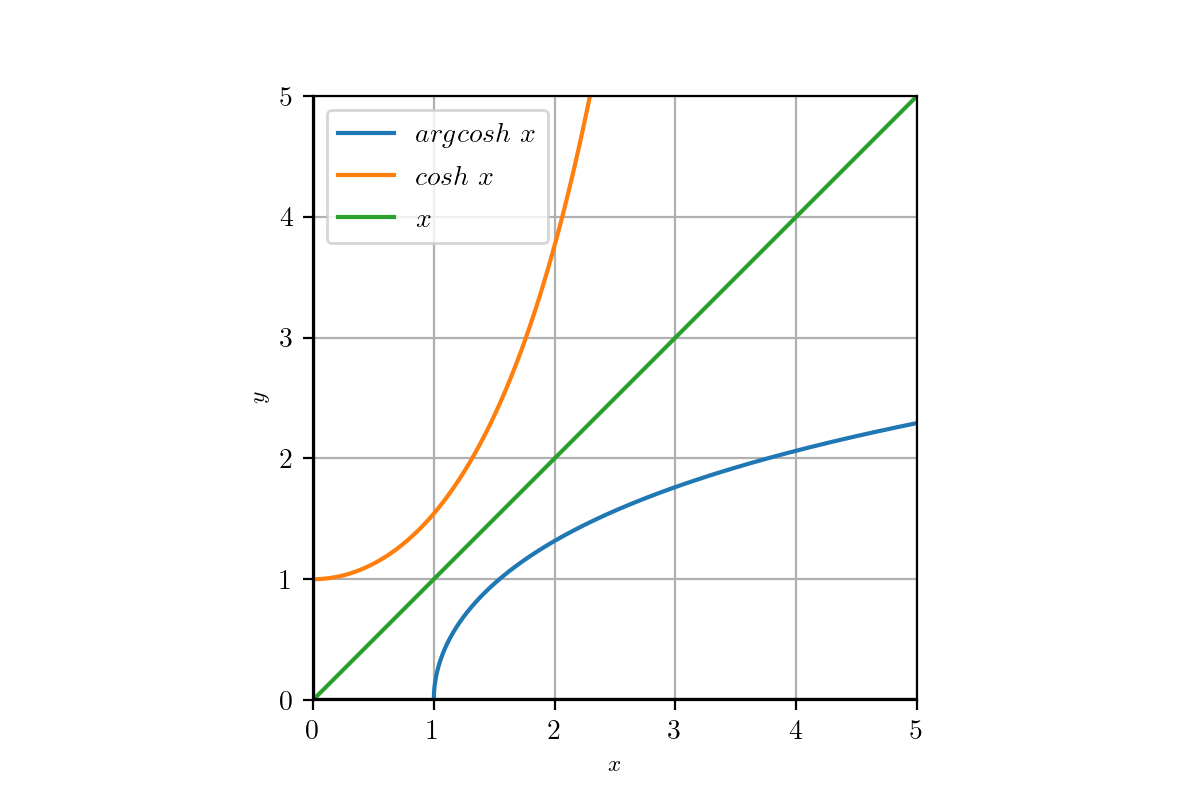
\includegraphics[scale=0.7]{argcosh.png}
  \caption{Tracé de fonctions hyperbolique \(\hcos\) et \(\argch\)}
  \label{fig:tracecoshargcosh}
\end{figure}
%
\subsection{Fonction argument tangente hyperbolique}
\label{subsec:chap1-fonctionargtanh}
\begin{defdef}
  La fonction tangente hyperbolique induit une bijection de \(\R\) sur \(\intervalleoo{-1}{1}\). Elle admet donc une réciproque appelée argument tangente hyperbolique notée \(\argth\).
\end{defdef}
%
\begin{prop}
  Pour tous réel \(x\) et \(y\) de \(\intervalleoo{-1}{1}\), on a
  \begin{gather}
    y=\htan x \iff x= \argth x, \\
    \argth(\htan x)=x, \\
    \htan(\argth y)=y.
  \end{gather}
\end{prop}
%
\begin{prop}
  La fonction argument tangente hyperbolique est impaire et strictement croissante.
\end{prop}
%
\begin{prop}
  La fonction argument tangente hyperbolique est dérivable sur son ensemble de définition telle que
  \begin{equation}
    \forall x \in \intervalleoo{-1}{1} \quad \argth'(x)=\frac{1}{1-x^2}.
  \end{equation}
\end{prop}
\begin{proof}
  Puisque tangente hyperbolique est dérivable sur \(\R\) et que
  \begin{equation}
    \htan'(\argth y)=1-\htan^2(\argth y)=1-y^2>0,
  \end{equation}
  alors la fonction \(\argth\) est dérivable et la formule est donnée.
\end{proof}
%
\begin{prop}[Expression logarithmique]
  La fonction argument tangente hyperbolique peut s'écrire telle que
  \begin{equation}
    \forall y \in \intervalleoo{-1}{1} \quad \argth y =\frac{1}{2} \ln \left( \frac{1+y}{1-y} \right).
  \end{equation}
\end{prop}
\begin{proof}
  \begin{equation}
    \forall (x,y) \in \R \times \intervalleoo{-1}{1} \quad y=\htan x = \frac{\e^{2x}-1}{\e^{2x}+1},
  \end{equation}
  de la même manière on arrive à une équation du deuxième degré~:
  \begin{equation}
    \e^{2x} = \frac{1+y}{1-y} ,
  \end{equation}
  et puisque \(-1<y<1\), on peut passer au logarithme et on obtient la formule.
\end{proof}
%
\begin{figure}
  \centering
  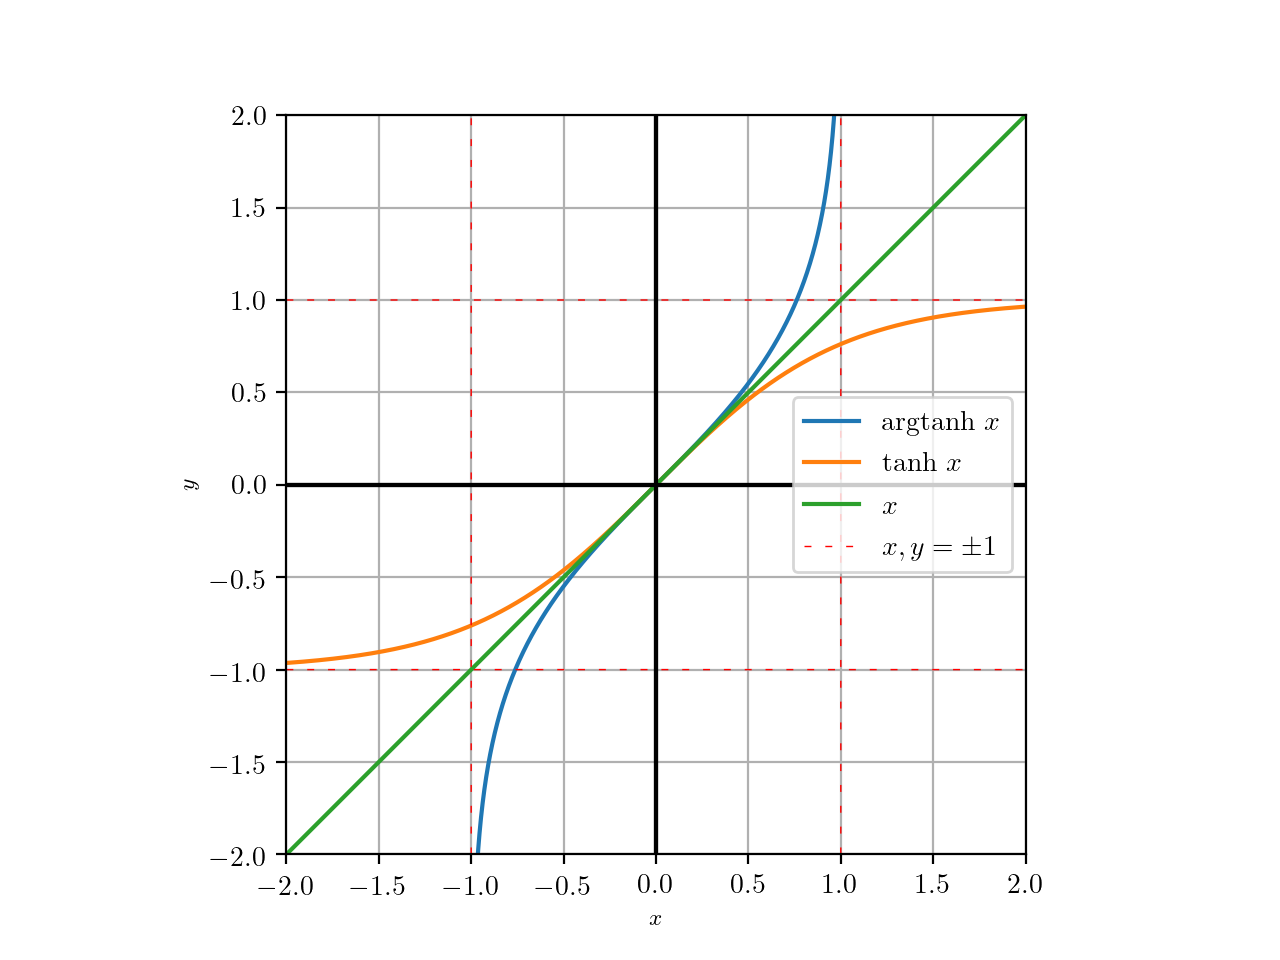
\includegraphics[scale=0.7]{argtanh.png}
  \caption{Tracé des fonctions hyperbolique \(\htan\) et \(\argth\) et de leurs asymptotes}
  \label{fig:tracetanhargth}
\end{figure}
\cleardoublepage
\section{Exercices --- Fonctions logarithme, exponentielle et puissances}
\begin{exercice}
    Soit \(a > 1\) et \(\alpha \in \R\).
    \begin{itemize}
        \item Discuter le nombre de racines sur \(\intervalleoo{0}{+\infty}\) de l'équation~:
            \begin{equation}
                \label{eq:fiche1-1}
                a^x = x^\alpha
            \end{equation}
        \item Démontrer que l'équation~:
            \begin{equation}
                a^{a^x} = x
            \end{equation}
            a les mêmes racines que l'équation~:
            \begin{equation}
                a^x = x.
            \end{equation}
            En déduire le nombre de racines de l'équation \eqref{eq:fiche1-1}.
    \end{itemize}
\end{exercice}
\begin{exercice}
    Résoudre sur \(\intervalleoo{0}{+\infty}\) le système d'équations aux inconnues \(x\) et \(y\) suivant~:
    \begin{equation}
       \begin{cases} 7(\log_y x +\log_x y) = 50 \\ xy = 256 \end{cases} 
    \end{equation}
\end{exercice}
\begin{exercice}
    Comparer \(\e^\pi\) et \(\pi^e\).
\end{exercice}
\begin{exercice}
    Soit, pour tout réel \(\alpha\) et tout naturel \(n\) non nul la fonction \(f_{alpha, n}\), notée par la suite $f$, définie pour tout \(x>0\), \(f_{\alpha, n}(x) = x^\alpha (\ln x)^n \).
    \begin{enumerate}
        \item Étudier la fonction \(f\) au voisinage de ses bornes
        \item Étudier les variations de \(f\)
        \item Représenter graphiquement \(f\). \emph{Attention, on devra trouver 15 représentations graphiques distinctes, en fonction de la valeur de \(n\) et de \(\alpha\).}
    \end{enumerate}
\end{exercice}
\begin{exercice}
    Résoudre dans \(\R\) les équations suivantes~:
    \begin{align}
        (\sqrt{x})^x &= x^{\sqrt{x}} \\
        2\ln x + \ln(2x-1) &= \ln(2x+8) + 2\ln(x-1) \\
        \e^{2x} -2\e^x-3 &=0 \\
        \sqrt{x+4-4\sqrt{x}} + \sqrt{x+9-6\sqrt{x}} &= 1
    \end{align}
\end{exercice}
\section{Exercice --- Fonctions circulaires, hyperboliques et leurs réciproques}
\begin{exercice}
    Résoudre sur \(\R\) l'équation~:
    \begin{equation}
        \frac{\sin x + \sin 2x + \sin 3x}{\cos x + \cos 2x + \cos 3x} = 1
    \end{equation}
\end{exercice}
\begin{exercice}
    Soit la fonction \(f\) telle que~:
    \begin{equation}
        f(x) = (\sqrt{1-\sin 2x}+\sqrt{1+\sin 2x})^{\frac{1}{\ln(\cos 2x)}}
    \end{equation}
    \begin{enumerate}
        \item Quel est le domaine de définition de \(f\) ?
        \item Démontrer que quelque soit le réel \(x\), \(\sqrt{1-\sin 2x}=\abs{\sin x - \cos x}\).
        \item Étudier la parité et la périodicité de \(f\)
        \item Trouver une expression de \(f\) plus simple sur \(\intervallefo{0}{\pi/2}\setminus\{\pi/3\}\).
        \item Étudier les variations de \(f\) et la représenter graphiquement.
    \end{enumerate}
\end{exercice}
\begin{exercice}
    Résoudre sur \(\R\) l'équation
    \begin{equation}
        2\arcsin x = \arcsin(2x\sqrt{1-x^2})
    \end{equation}
\end{exercice}
\begin{exercice}
    Déterminer pour tout réel \(a\) et tout naturel \(n\) une expression simple de la somme~:
    \begin{equation}
        S_n = \sum_{k=1}^n 2^k \tanh(2^k a
    \end{equation}
    \emph{Indication :} On pourra essayer de simplifier l'expression~:
    \[\frac{2}{\tanh 2x} - \frac{1}{\tanh x}\]
\end{exercice}
\begin{exercice}
    Déterminer, pour tout réel \(x\) de l'intervalle \(\intervallefo{0}{\pi/2}\) et tout naturel \(n\), une expression simple du réel~:
    \begin{equation}
        \sum_{k=0}^{n-1} \frac{\cos kx}{\cos^k x}
    \end{equation}
\end{exercice}
\begin{exercice}
    Déterminer si elles existent les limites~:
    \begin{align}
        \lim\limits_{x \to +\infty} 2\cosh^2x-\sinh 2x \\
        \lim\limits_{x \to +\infty} \e^{2x}(2\cosh^2x-\sinh 2x)
    \end{align}
\end{exercice}
\begin{exercice}
    Soient \(y \in \intervalleoo{0}{\pi/2}\) et \(x = \ln\tan(\pi/4+y/2)\). Exprimer en focntion de \(y\) chacun des réels \(\tanh(x/2), \sinh x, \cosh x\) et \(\tanh x\).
\end{exercice}
\begin{exercice}
    Démontrer que pour tout réels \(a\) et \(b\) strictement compris entre \(-1\) et \(1\),
    \begin{equation}
        \argth a + \argth b = \argth \frac{a+b}{1+ab}
    \end{equation}
\end{exercice}
\begin{exercice}
    Soient \(a\) et \(b\) deux réels. Résoudre sur \(\R\) le système suivant~:
    \begin{equation}
        \begin{cases} \cosh x \cosh y = a \\ \sinh x \sinh y = b \end{cases}
    \end{equation}
\end{exercice}
\begin{exercice}
    Étudier et représenter graphiquement les fonctions \(f\) suivantes~:
    \begin{align}
        f(x) &= \arcsin \sin x \\
        f(x) &= \argch \sqrt{\frac{1+\cosh x}{2}} \\
        f(x) &= \arccos(4x^3-3x) \\
        f(x) &= \argth\sqrt{\frac{\cosh x - 1}{\cosh x + 1}}
    \end{align}
\end{exercice}
\begin{exercice}
    Soit un réel \(x\), simplifier l'expression~:
    \begin{equation}
        \arccos \cos x + 1/2 \arccos\cos 2x + 1/6\arccos\cos 3x
    \end{equation}
\end{exercice}
\begin{exercice}
    Soit un réel \(x\), comparer \(\cos\sin x\) et \(\sin\cos x\).
\end{exercice}
